\chapter{膜电位和神经元的被动电特性} \label{chap:chap9}

信息在神经元内部以及通过电信号和化学信号从神经元传送到它们的靶细胞。
瞬态电信号对于快速和远距离传输时间敏感信息尤为重要。
这些瞬态电信号——受体电位、突触电位和动作电位——都是由进出细胞的电流的暂时变化产生的,这些变化驱动细胞膜上的电位远离其静止值。
该电流代表通过细胞膜中离子通道的负离子和正离子的流动。


两种类型的离子通道——静息和门控——在神经元信号传导中具有独特的作用。
静息通道在维持静息膜电位方面非常重要,静息膜电位是在没有信号的情况下跨膜的电位。
某些类型的静息通道是结构性开放的,不受膜电压变化的限制;
其他类型由电压变化门控,但也在神经元的负静息电位下打开。
相反,大多数电压门控通道在膜静止时关闭,需要膜去极化才能打开。


在本章和接下来的几章中,我们将考虑瞬态电信号是如何在神经元中产生的。
我们首先讨论特定离子通道如何在膜静止时建立和维持膜电位,并简要描述静息电位可能受到干扰的机制,从而产生瞬态电信号,例如动作电位。
然后我们考虑神经元的被动电特性——它们的电阻和电容特性——如何促进神经元内突触和受体电位的整合和局部传播。
在第~\ref{chap:chap10}~章中,我们研究了电压门控 \ce{Na+}、\ce{K+} 和 \ce{Ca^2+} 通道产生动作电位的详细机制,动作电位是沿轴突传递的电信号。
突触电位在第~\ref{chap:chap11}~章到第 ~\ref{chap:chap14}~章中讨论,受体电位在第 IV 部分与感觉受体的作用相关讨论。



\section{跨细胞膜的电荷分离产生静息膜电位}

神经元的细胞膜有薄薄的正离子和负离子云散布在其内外表面。
静止时,膜的细胞外表面有过量的正电荷,而细胞质表面有过量的负电荷(图~\ref{fig:9_1})。
这种电荷分离得以维持是因为膜的脂质双层是离子扩散的屏障(第~\ref{chap:chap8}~章)。
电荷分离产生膜电位 (Vm),跨膜的电位差或电压,定义为:
\begin{equation}
	V_m = V_{in} - V_{out},
\end{equation}
其中 Vin 是电池内部的电位,Vout 是外部的电位。


静止细胞的膜电位,即静止膜电位 (Vr),等于 Vin,因为按照惯例,细胞外的电位被定义为零。
其通常范围为 −60 mV 至 −70 mV。
所有电信号都涉及由跨细胞膜的电流引起的远离静息膜电位的短暂变化。


\begin{figure}[htbp]
	\centering
	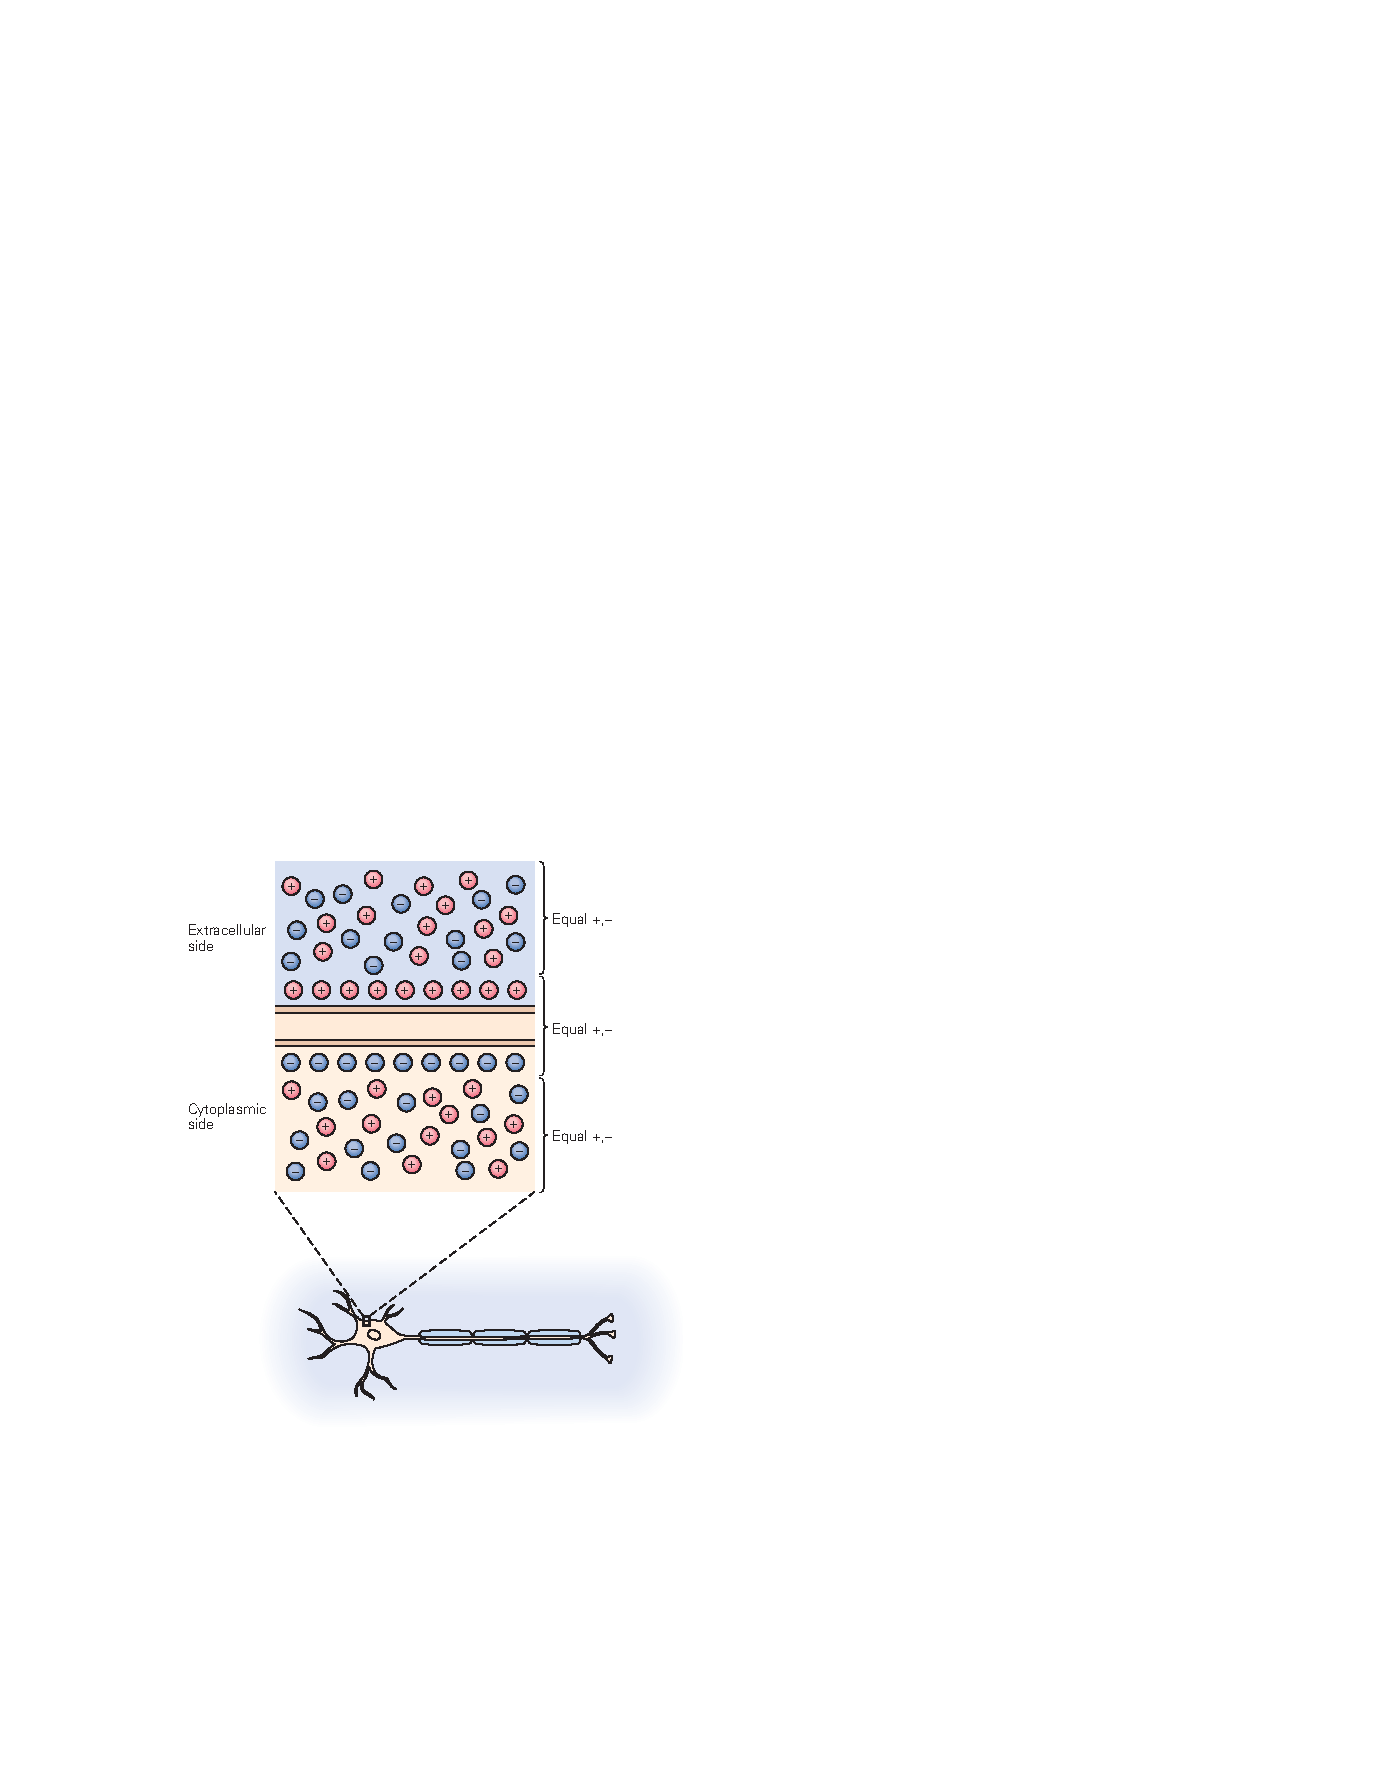
\includegraphics[width=0.5\linewidth]{chap09/fig_9_1}
	\caption{细胞膜电位是由膜两侧的净正电荷和净负电荷分离产生的。 膜外过量的正离子和膜内的负离子占静止细胞内外离子总数的一小部分。}
	\label{fig:9_1}
\end{figure}


电流由正离子(阳离子)和负离子(阴离子)携带。
电流的方向通常定义为正电荷净移动的方向。
因此,在离子溶液中,阳离子沿电流方向移动,阴离子沿相反方向移动。
在静止的神经细胞中,跨膜没有净电荷运动。
当阳离子或阴离子净流入或流出细胞时,静息膜上的电荷分离会受到干扰,从而改变膜的电势。
电荷分离的减少或逆转,导致较低的负膜电位,称为去极化。
电荷分离的增加导致更负的膜电位,称为超极化。


不会导致门控离子通道打开的膜电位变化是膜的被动反应,称为电紧张电位。
超极化反应几乎总是被动的,小的去极化也是如此。
然而,当去极化接近临界水平或阈值时,细胞会积极响应电压门控离子通道的打开,从而产生全或无动作电位(方框~\ref{box:9_1})。


\begin{proposition}[记录膜电位] \label{box:9_1}
	
	\quad \quad 20世纪40年代末,开发了可靠的记录细胞膜电位的技术。
	这些技术可以准确记录静息膜电位和动作电位(图~\ref{fig:9_2})。
	
	\quad \quad 充满浓盐溶液的玻璃微量移液器用作电极,并放置在细胞膜的任一侧。
	插入移液管后端的电线通过放大器连接到示波器,示波器以伏特为单位显示膜电位的幅度。
	由于这种微电极尖端的直径很小(<1μm),因此可以将其插入细胞中,而对细胞膜的损伤相对较小(图~\ref{fig:9_2}A)。
	
	\quad \quad 当两个电极都在电池外部时,不会记录电位差。
	但一旦将一个微电极插入电池,示波器就会显示出稳定的电压,即静息膜电位。
	在大多数静止的神经细胞中,膜电位约为-65 mV(图~\ref{fig:9_2}B)。
	
	\quad \quad 可以使用连接到第二对电极(一个细胞内电极和一个细胞外电极)的电流发生器通过实验改变膜电位。
	当细胞内电极相对于细胞外电极呈阳性时,来自电流发生器的正电流脉冲导致正电荷从细胞内电极流入神经元。
	该电流通过膜向外流动返回细胞外电极。
	
	\quad \quad 结果,膜的内部变得更加积极,而膜的外部变得更加消极。
	电荷分离的这种减少称为\textit{去极化}。
	
	\quad \quad 小的去极化电流脉冲在电池中引起纯电(被动)电位。
	电位变化的大小与电流脉冲的大小成正比。
	然而,足够大的去极化电流会触发电压门控离子通道的打开。
	这些通道的打开会产生动作电位,动作电位的产生方式以及幅度和持续时间都不同于电离子电位(图~\ref{fig:9_2}C)。
	
	\quad \quad 反转电流方向,使细胞内电极相对于细胞外电极负,使膜电位更负。
	这种电荷分离的增加被称为\textit{超极化}。
	
	\quad \quad 超极化不会触发细胞中的主动反应。
	细胞对超极化的反应通常是纯电张力的。
	随着电流脉冲大小的增加,超极化成比例地增加(图~\ref{fig:9_2}D)。
	
\end{proposition}


\begin{figure}[htbp]
	\centering
	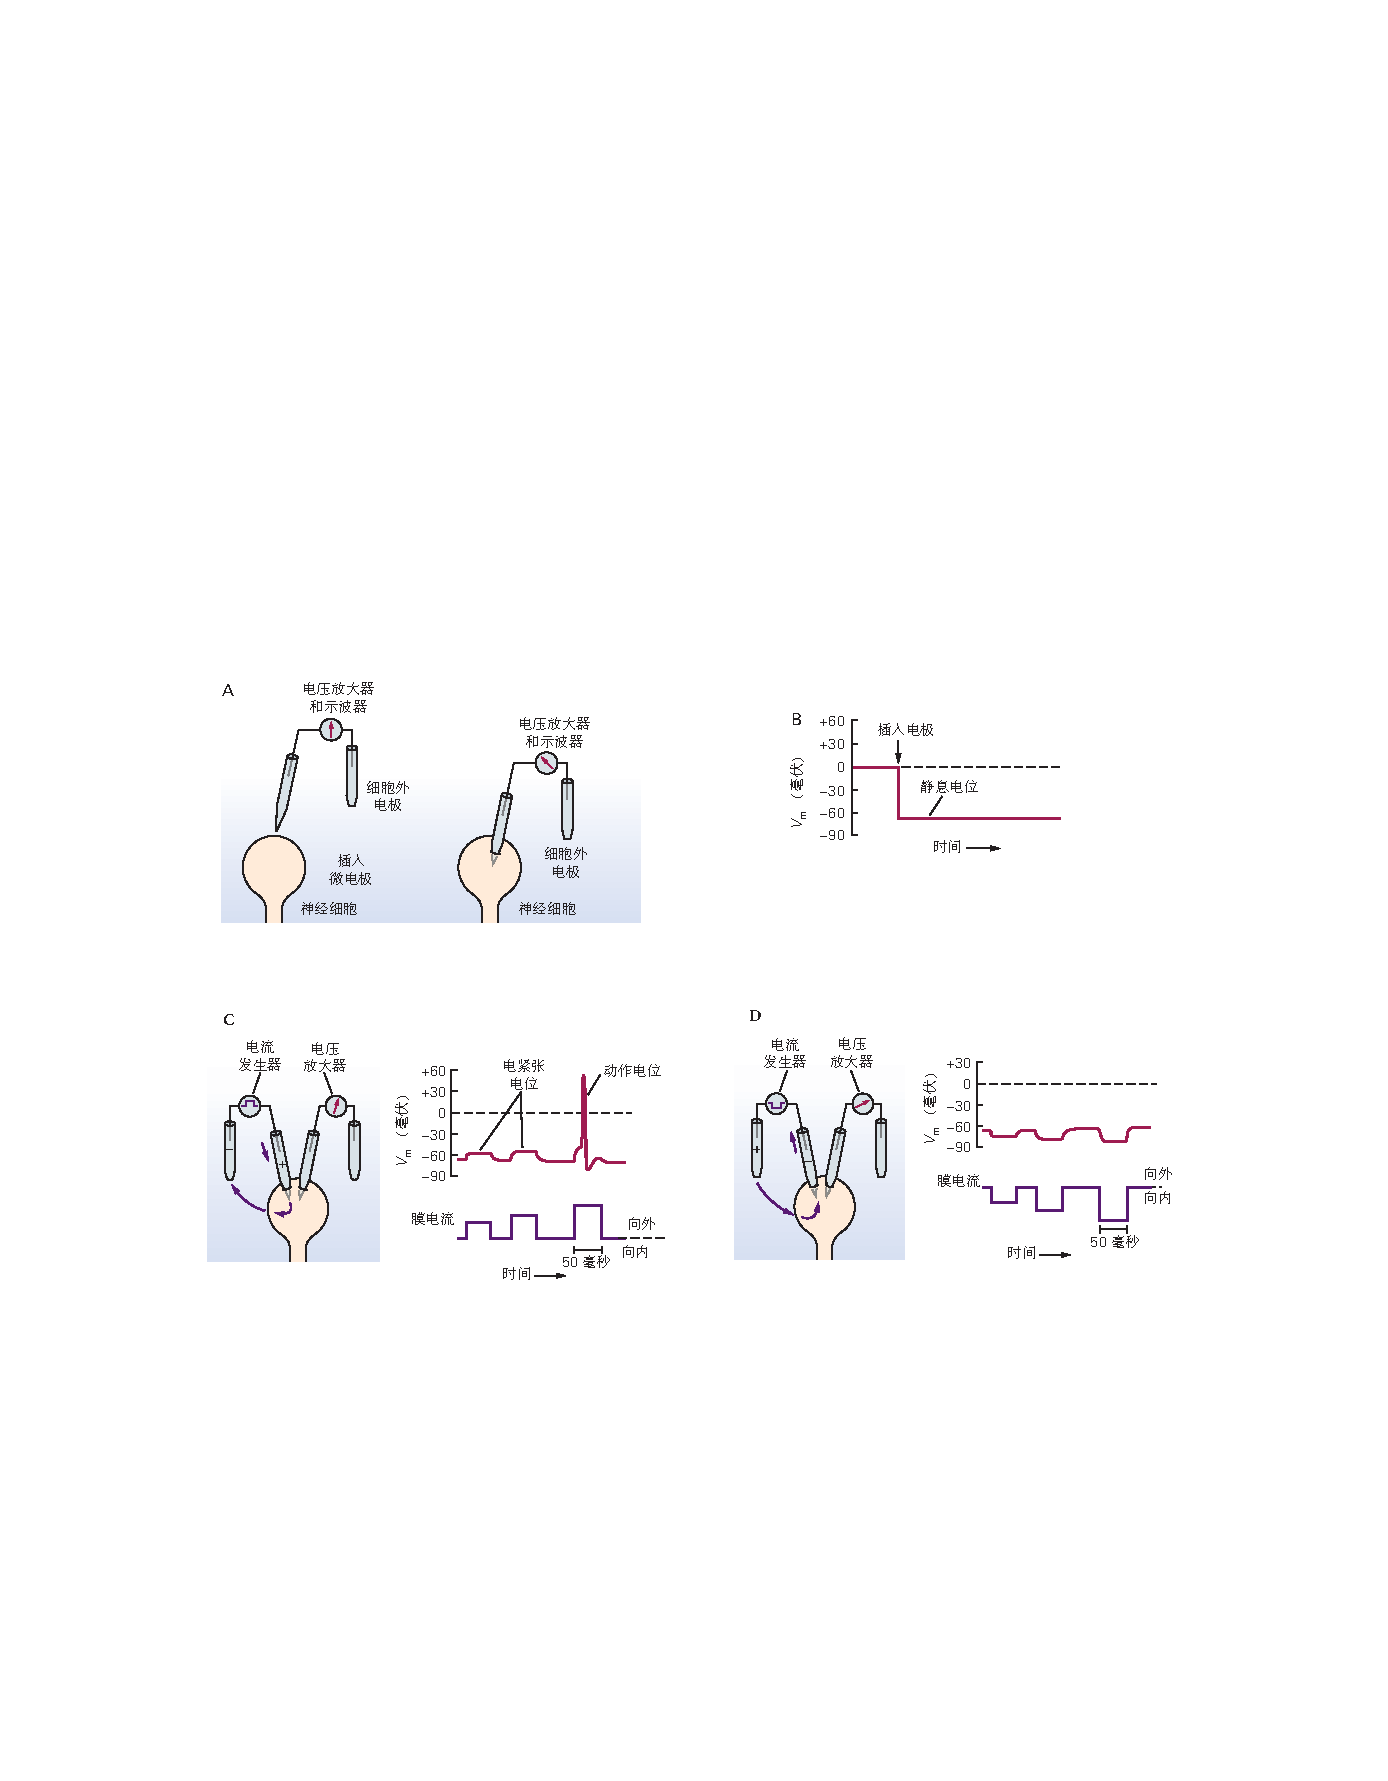
\includegraphics[width=0.8\linewidth]{chap09/fig_9_2}
	\caption{\textbf{A.} 记录设置。
	\textbf{B.} 示波器显示。
	\textbf{C.} 去极化。
	\textbf{D.} 超极化。}
	\label{fig:9_2}
\end{figure}



\section{静息膜电位由非门控和门控离子通道决定}

静息膜电位是单个离子种类通过几类静息通道的被动通量的结果。
了解这种被动离子通量如何产生静息电位,使我们能够了解不同类型离子通道的门控如何产生动作电位,以及受体和突触电位。


没有单一的离子种类均匀分布在神经细胞膜的两侧。
在细胞膜两侧发现的四种最丰富的离子中,\ce{Na+} 和 \ce{Cl-} 集中在细胞外,\ce{K+} 和 A-(有机阴离子,主要是氨基酸和蛋白质)集中在细胞内。
表 9-1 显示了这些离子在一个经过特别深入研究的神经细胞过程内外的分布,即鱿鱼的巨大轴突,其细胞外液的盐浓度与海水相似。
尽管脊椎动物神经细胞的离子浓度绝对值比乌贼巨型轴突低两到三倍,但浓度梯度(外部离子浓度与内部离子浓度之比)相似。


离子的不均匀分布引发了几个重要问题。
离子梯度如何影响静息膜电位?
是什么阻止离子梯度因离子通过静息通道跨膜扩散而消散?
这些问题是相互关联的,我们将通过考虑膜渗透性的两个例子来回答它们:胶质细胞的静息膜只能渗透一种离子,神经细胞的静息膜可以渗透三种离子。
出于本次讨论的目的,我们将只考虑不受电压门控并因此始终打开的静止通道。



\subsection{神经胶质细胞中的开放通道仅可渗透钾}

细胞膜对特定离子种类的渗透性取决于各种类型的开放离子通道的相对比例。
最简单的情况是神经胶质细胞,其静息电位约为 -75 mV。
与大多数细胞一样,神经胶质细胞内部具有高浓度的 \ce{K+} 和 A-,而外部具有高浓度的 \ce{Na+} 和 \ce{Cl-}。
然而,膜中的大多数静息通道仅可渗透 \ce{K+}。


由于 \ce{K+} 离子在细胞内以高浓度存在,因此它们倾向于沿着其化学浓度梯度从细胞内扩散到细胞外。
结果,膜的外部积聚了净正电荷(由 \ce{K+} 略微过量引起),而内部则积聚了净负电荷(由于 \ce{K+} 不足和由此产生的阴离子略微过量)。
由于相反的电荷相互吸引,外部多余的正电荷和内部多余的负电荷局部聚集在膜的任一表面(图 9–1)。


\ce{K+} 流出细胞是自限性的。
\ce{K+} 的流出会产生电位差——外部为正,内部为负。
\ce{K+} 的流量越大,分离的电荷越多,电位差就越大。
因为\ce{K+}是正的,细胞内的负电位往往会阻止\ce{K+}的进一步流出。
因此,\ce{K+} 离子受到驱动它们穿过膜的两种力:(1) 化学驱动力,跨膜浓度梯度的函数,以及 (2) 电驱动力,跨膜电位差的函数 膜。


一旦 \ce{K+} 扩散进行到某个点,\ce{K+} 上的电驱动力恰好平衡了化学驱动力。
也就是说,\ce{K+} 的向外运动(由其浓度梯度驱动)等于 \ce{K+} 的向内运动(由跨膜电势差驱动)。
该电位称为 \ce{K+} 平衡电位 EK(图~\ref{fig:9_3})。
在仅可渗透 \ce{K+} 离子的细胞中,EK 决定静息膜电位,在大多数神经胶质细胞中约为 -75 mV。


\begin{figure}[htbp]
	\centering
	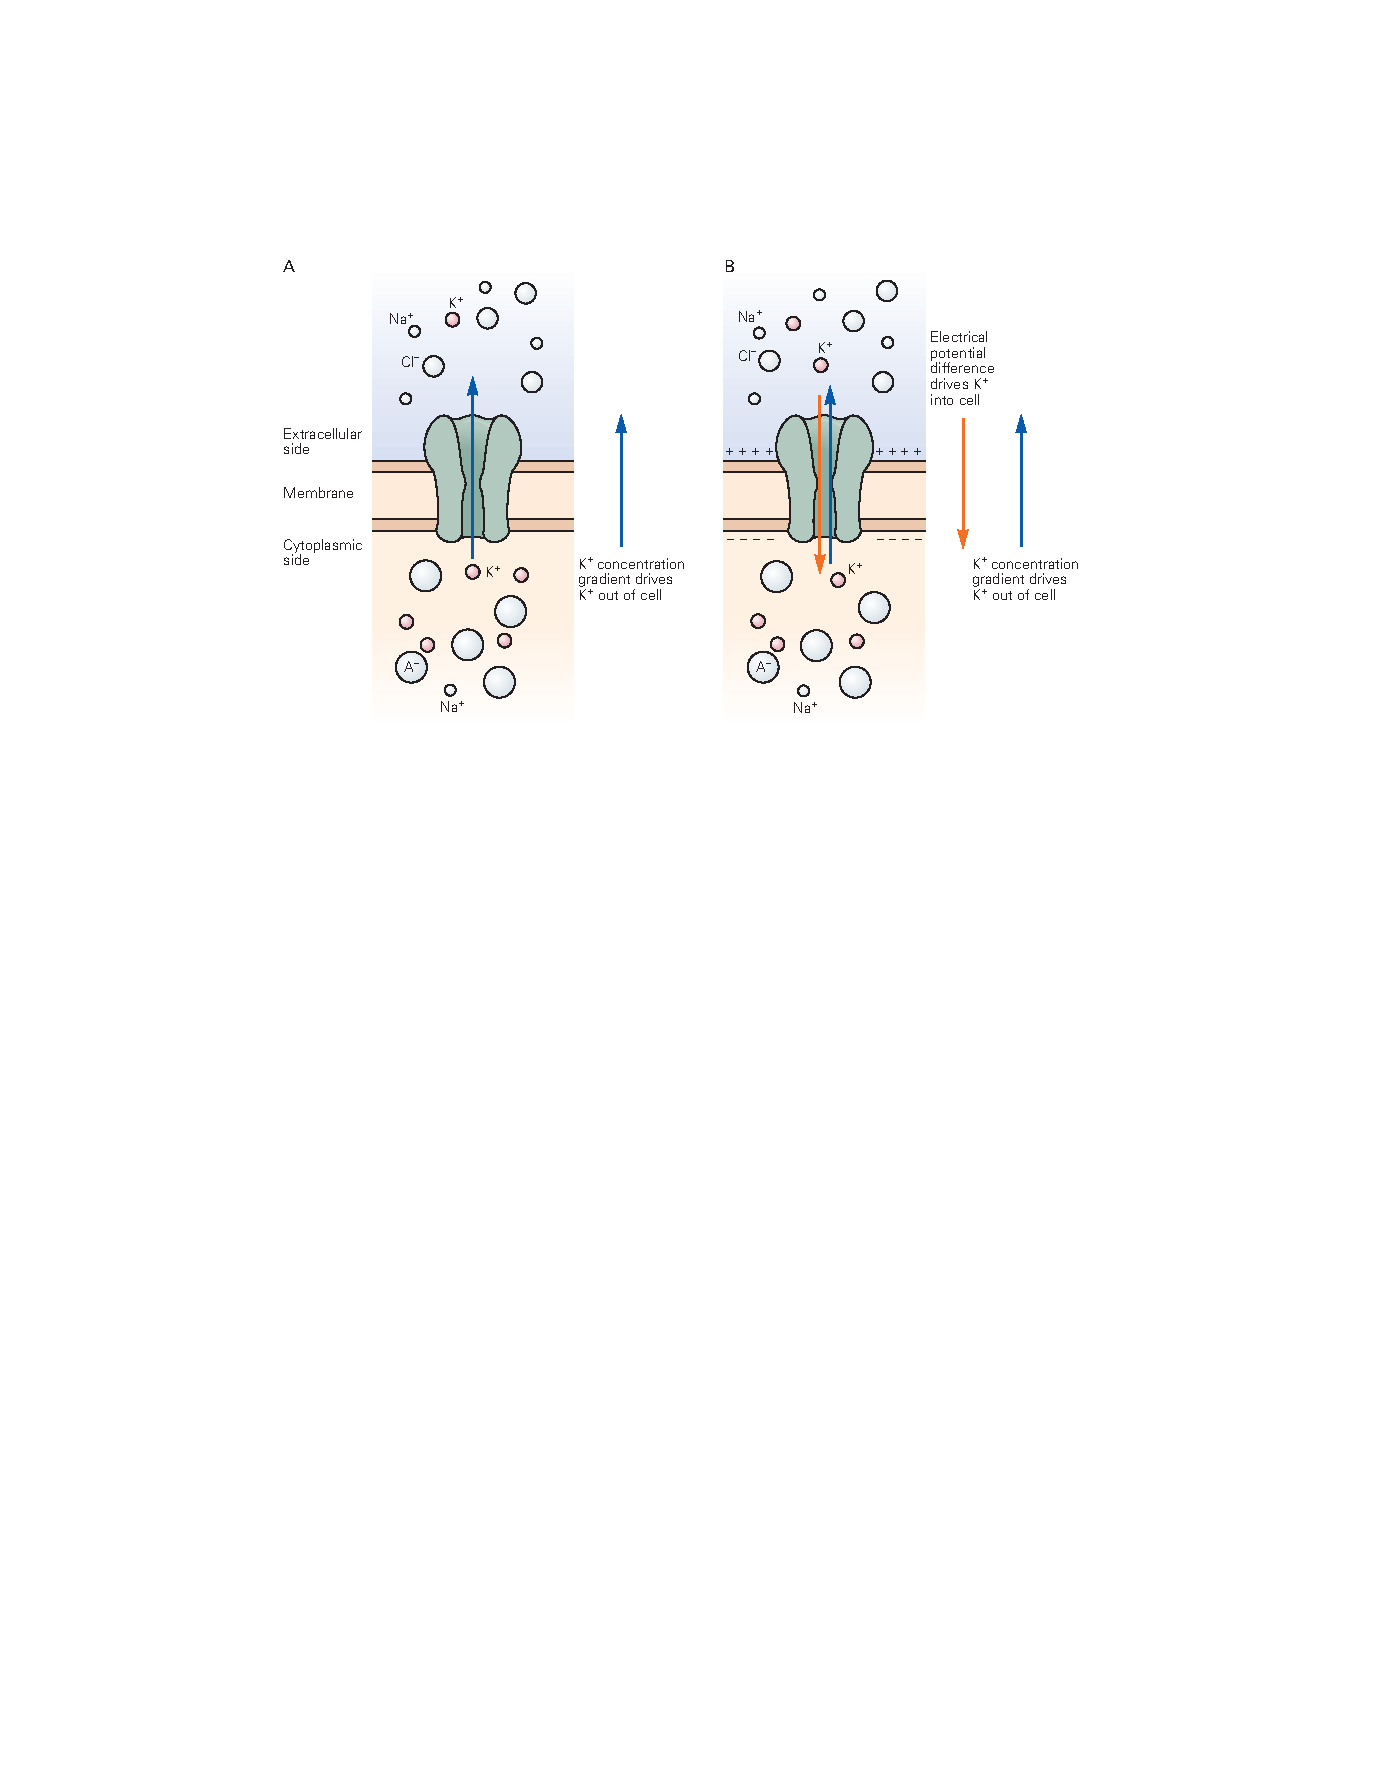
\includegraphics[width=0.7\linewidth]{chap09/fig_9_3}
	\caption{\ce{K+} 穿过细胞膜的通量由 \ce{K+} 浓度梯度和膜电位共同决定。 A. 在只对 \ce{K+} 具有渗透性的细胞中,静息电位是由 \ce{K+} 沿着其浓度梯度流出产生的。 B. \ce{K+} 的持续流出在细胞外部积累了过多的正电荷,并在细胞内部留下了过多的负电荷。 这种电荷的积累导致跨膜的电位差阻碍 \ce{K+} 的进一步流出,因此最终达到平衡:电驱动力和化学驱动力相等且相反,因此有多少 \ce{K+} 离子移入和移出。}
	\label{fig:9_3}
\end{figure}


任何离子 X 的平衡电位都可以根据德国物理化学家沃尔特能斯特 (Walter Nernst) 于 1888 年根据基本热力学原理推导出的方程式计算:


其中 R 是气体常数,T 是温度(以开氏度为单位),z 是离子的化合价,F 是法拉第常数,[X]o 和 [X]i 是电池内外的离子浓度。
(准确地说,应使用化学活度而不是浓度。)


由于 RT/F 在 25°C(77°F,室温)时为 25 mV,并且自然对数转换为以 10 为底的对数的常数为 2.3,因此 Nernst 方程也可以写成如下形式:


因此,对于 \ce{K+},由于 z = +1 并给定表 9-1 中鱿鱼轴突内外的浓度:


能斯特方程可用于找到存在于可渗透该离子的膜两侧的任何离子的平衡电位(该电位有时称为能斯特电位)。
表 9-1 给出了 \ce{Na+}、\ce{K+} 和 \ce{Cl-} 离子在鱿鱼巨型轴突上的分布平衡电位。


到目前为止,在我们的讨论中,我们将静息电位的产生视为一种被动机制——离子沿其化学梯度扩散——一种不需要细胞消耗能量的机制。
然而,需要来自三磷酸腺苷 (ATP) 水解的能量来建立初始浓度梯度并在神经元中维持它们,正如我们将在下面看到的。



\subsection{静息神经细胞中的开放通道可渗透三种离子}

与神经胶质细胞不同,除了 \ce{K+} 离子外,静止的神经细胞还可以渗透 \ce{Na+} 和 \ce{Cl-} 离子。
在神经细胞中丰富的离子种类中,只有大的有机阴离子 (A−) 无法渗透细胞膜。
三种渗透性离子(\ce{Na+}、\ce{K+} 和 \ce{Cl-})的浓度梯度如何在单个细胞的膜上保持不变,这三个梯度如何相互作用以确定细胞的静息膜电位?


要回答这些问题,首先只检查 \ce{K+} 和 \ce{Na+} 的扩散是最简单的。
让我们回到只有 \ce{K+} 通道的细胞的简单示例,\ce{K+}、\ce{Na+}、\ce{Cl-} 和 A- 的浓度梯度如表 9-1 所示。
在这些条件下,静息膜电位 Vr 仅由 \ce{K+} 浓度梯度决定,等于 EK (−75 mV)(图~\ref{fig:9_4} A)。


\begin{figure}[htbp]
	\centering
	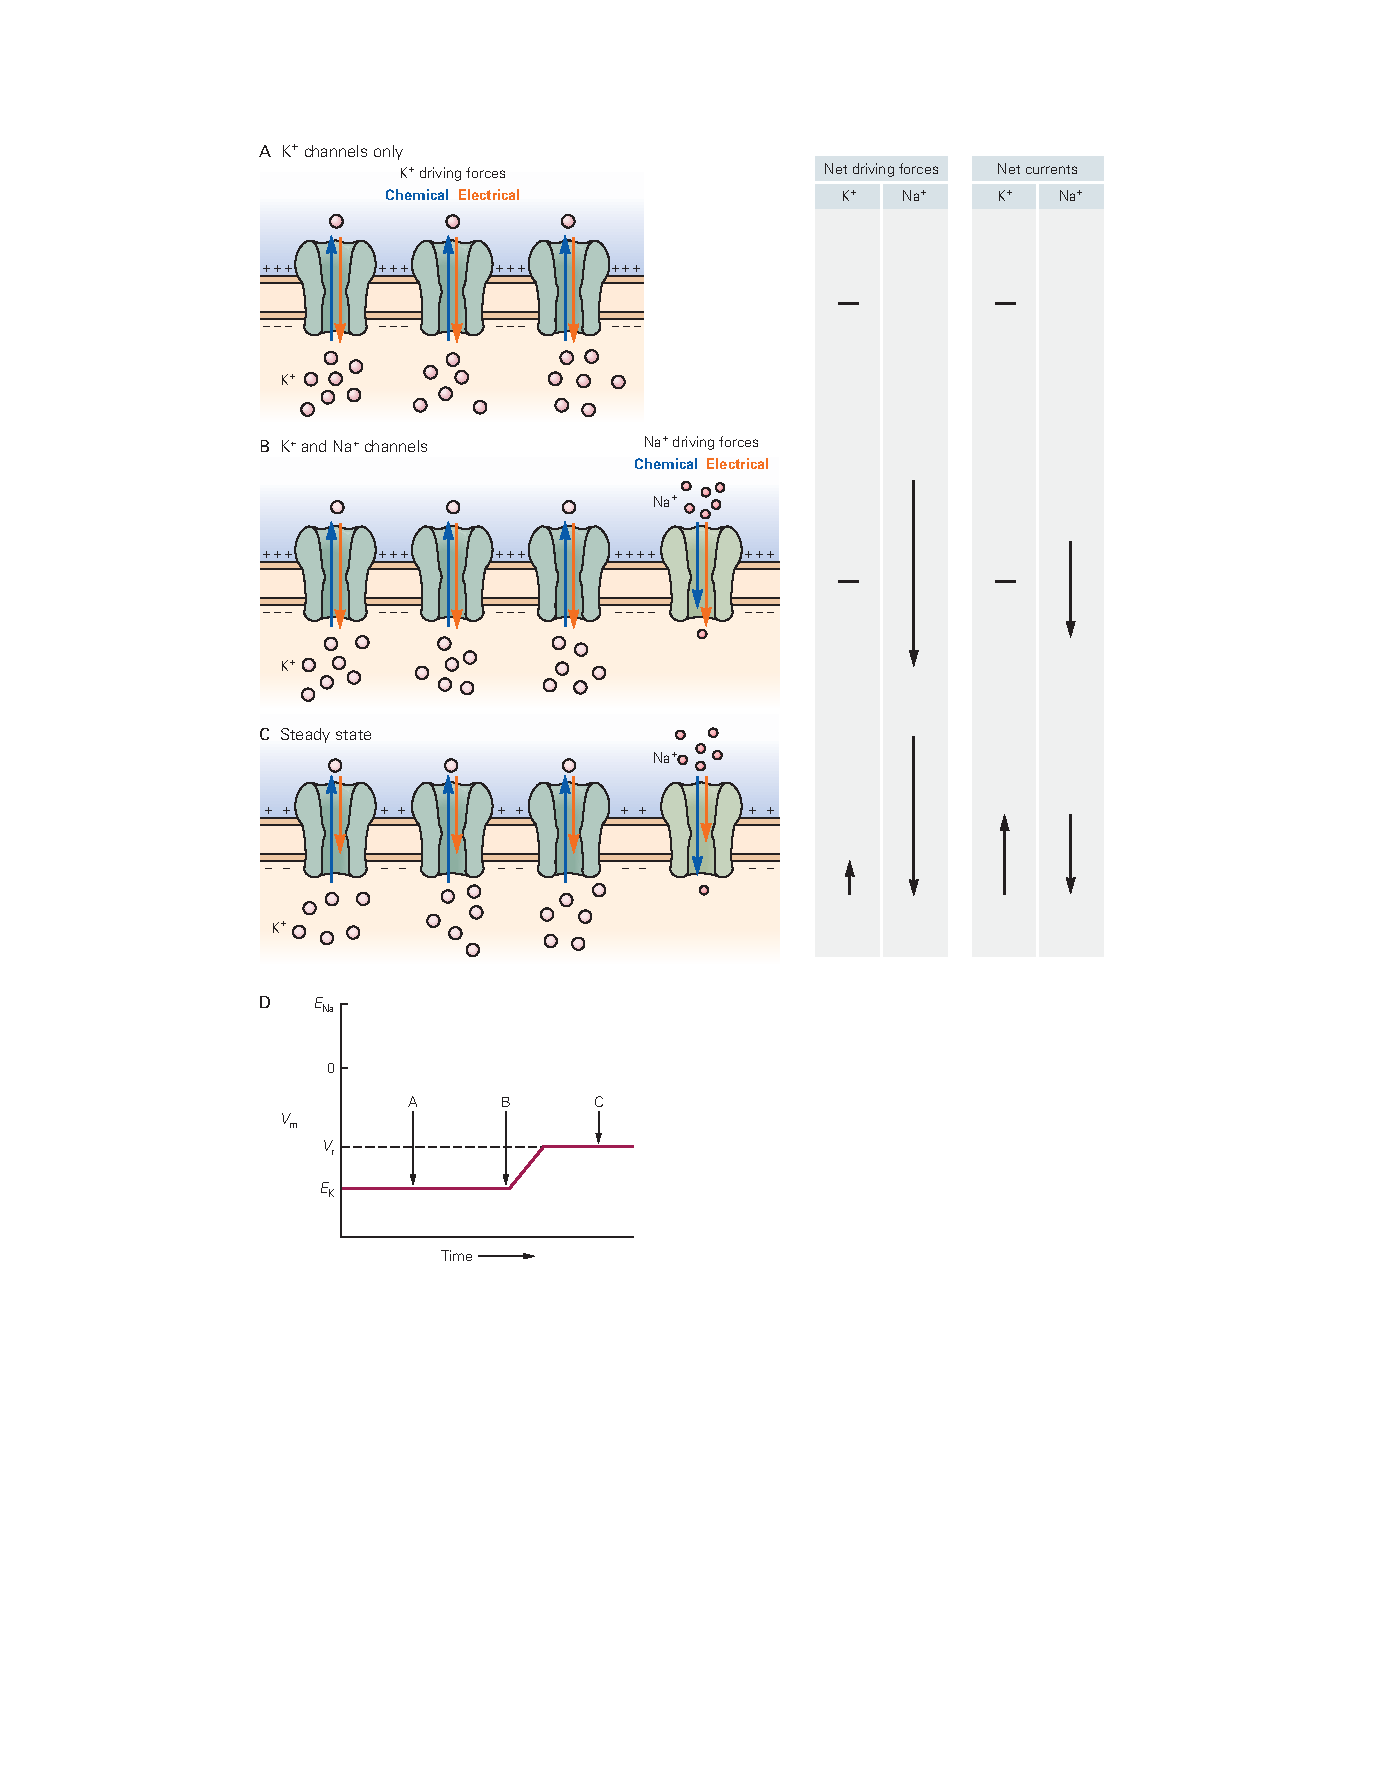
\includegraphics[width=0.7\linewidth]{chap09/fig_9_4}
	\caption{细胞的静息电位由开放的不同类型离子通道的比例及其平衡电位值决定。 图中的通道代表了这个假设的细胞膜中完整的 \ce{K+} 或 \ce{Na+} 通道。 通道内箭头的长度表示作用于 \ce{Na+} 或 \ce{K+} 的电(红色)和化学(蓝色)驱动力的相对振幅。 右图中箭头的长度表示 \ce{Na+} 和 \ce{K+} 的净驱动力(电驱动力和化学驱动力的总和)和净离子电流的相对大小。 说明了三种假设情况。 A. 在仅存在 \ce{K+} 通道的静息细胞中,\ce{K+} 离子处于平衡状态且 Vm = EK。 B. 向静息膜添加一些 \ce{Na+} 通道可使 \ce{Na+} 离子扩散到细胞中,这种流入开始使膜去极化。 C. 静息电位稳定在一个新水平 (Vr),此时 \ce{Na+} 的流入与 \ce{K+} 的流出平衡。 在此示例中,\ce{K+} 通道的总电导远大于 \ce{Na+} 通道的总电导,因为 \ce{K+} 通道数量更多。 结果,相对较小的 \ce{K+} 净驱动力驱动的电流与由更大的 \ce{Na+} 净驱动力驱动的 \ce{Na+} 电流相等且相反。 这是一个稳态条件,其中 \ce{Na+} 和 \ce{K+} 都不处于平衡状态,但电荷的净通量为零。 D. 在 A、B 和 C 部分所示的假设情况下膜电压发生变化。}
	\label{fig:9_4}
\end{figure}


现在考虑如果在膜上添加一些静止的 \ce{Na+} 通道,使其对 \ce{Na+} 具有轻微的渗透性,会发生什么情况。
有两种力量将 \ce{Na+} 驱动到细胞中:\ce{Na+} 倾向于沿着其化学浓度梯度流入细胞,并通过跨膜的负电位差驱动进入细胞(图~\ref{fig:9_4} B)。
\ce{Na+} 的流入使细胞去极化,但仅略微偏离 \ce{K+} 平衡电位 (-75 mV)。
新的膜电位不会接近 +55 mV 的 \ce{Na+} 平衡电位,因为膜中的静息 \ce{K+} 通道比 \ce{Na+} 通道多得多。


一旦膜电位开始从 \ce{K+} 平衡电位值去极化,\ce{K+} 通量就不再跨膜处于平衡状态。
驱动 \ce{K+} 进入细胞的电力减少意味着现在有 \ce{K+} 净流出细胞,趋向于抵消 \ce{Na+} 流入。
膜电位去极化并远离 \ce{K+} 平衡电位越多,将 \ce{K+} 驱出细胞的净电化学力就越大,因此净 \ce{K+} 流出量也越大。
最终,膜电位达到一个新的静息水平,此时 \ce{K+} 向外运动的增加恰好平衡了 \ce{Na+} 的向内运动(图~\ref{fig:9_4} C)。
该平衡点(通常约为 −65 mV)远离 \ce{Na+} 平衡电位 (+55 mV),仅略高于 \ce{K+} 平衡电位 (-75 mV)。


要了解这个平衡点是如何确定的,请记住离子穿过细胞膜的通量大小是其电化学驱动力(电驱动力和化学驱动力的总和)与膜电导率的乘积 离子:


在静息神经细胞中,开放的 \ce{Na+} 通道相对较少,因此 \ce{Na+} 的膜电导非常低。
因此,尽管驱动 \ce{Na+} 进入细胞的化学力和电力很大,但 \ce{Na+} 的流入量很小。
相反,许多\ce{K+}通道在静息细胞的膜中是开放的,因此\ce{K+}的膜电导相对较大。
由于静止细胞中 \ce{K+} 相对于 \ce{Na+} 的高电导率,作用在 \ce{K+} 上的小的净向外力足以产生与 \ce{Na+} 内流相等的 \ce{K+} 外流。



\subsection{钠、钾和钙的电化学梯度是由离子的主动传输建立的}

正如我们所见,\ce{K+} 通过开放通道被动移出静息细胞平衡了 \ce{Na+} 被动移入细胞。
然而,这种稳定的离子泄漏不能在任何可感知的时间长度内不受阻碍地继续,因为 \ce{Na+} 和 \ce{K+} 梯度最终会下降,从而降低静息膜电位。


钠-钾泵(\ce{Na+}-\ce{K+} 泵)阻止了离子梯度的消散,它使 \ce{Na+} 和 \ce{K+} 逆着它们的电化学梯度移动:
它从细胞中挤出 \ce{Na+},同时吸收 \ce{K+}。
因此,泵需要能量,而能量来自 ATP 的水解。
因此,在静息膜电位下,细胞不处于平衡状态,而是处于稳定状态:\ce{Na+} 持续被动流入,\ce{K+} 通过静息通道持续被动流入,这恰好被 \ce{Na+}-\ce{K+} 泵抵消。


正如我们在上一章中看到的,泵类似于离子通道,因为它们催化离子穿过细胞膜的运动。
然而,它们在两个重要方面有所不同。
首先,虽然离子通道是允许离子沿其电化学梯度向下移动的被动管道,但泵需要化学能源来逆着其电化学梯度传输离子。
其次,离子在通道中的传输速度要快得多:
离子通常以每秒 107 到 108 次的速度流过通道,而泵的运行速度要慢 10,000 多倍。


\ce{Na+}-\ce{K+} 泵是一种大型跨膜蛋白,其细胞内表面具有 \ce{Na+} 和 ATP 的催化结合位点,细胞外表面具有 \ce{K+} 的催化结合位点。
在每个循环中,泵都会水解一个 ATP 分子。
(因为 \ce{Na+}-\ce{K+} 泵水解 ATP,它也被称为 \ce{Na+}-\ce{K+} ATP 酶。)它利用这种水解能量从细胞中挤出三个 \ce{Na+} 离子并带入两个 \ce{K+} 离子。
\ce{Na+} 和 \ce{K+} 离子的不等通量导致泵产生净向外离子电流。
因此,泵被称为生电的。
这种由泵驱动的正电荷流出往往会使静息电位比前面讨论的被动扩散机制所达到的电位低几毫伏。
在神经元活动剧烈期间,\ce{Na+} 内流增加导致 \ce{Na+}-\ce{K+} 泵活动增加,从而产生延长的外向电流,导致持续几分钟的超极化后电位,直到恢复正常的 \ce{Na+} 浓度。
哇巴因或洋地黄植物生物碱可抑制 \ce{Na+}-\ce{K+} 泵,这种作用对治疗心力衰竭很重要。


\ce{Na+}-\ce{K+} 泵是称为 P 型 ATP 酶的一大类泵中的一员(因为 ATP 的磷酰基暂时转移到泵)。
P 型 ATP 酶包括一个钙离子泵,可跨细胞膜转运钙离子(图~\ref{fig:9_5}A)。
所有细胞通常都保持非常低的细胞质钙离子浓度,介于 50 和 100 nM 之间。
该浓度比外部浓度低四个数量级以上,在哺乳动物中约为 2 mM。
质膜中的钙泵将钙离子转运出细胞;
其他位于内膜的钙离子泵,例如光滑的内质网,将钙离子从细胞质转运到这些细胞内钙离子库中。
钙泵被认为为每个水解的 ATP 分子输送两个钙离子离子,两个质子沿相反方向输送。


\begin{figure}[htbp]
	\centering
	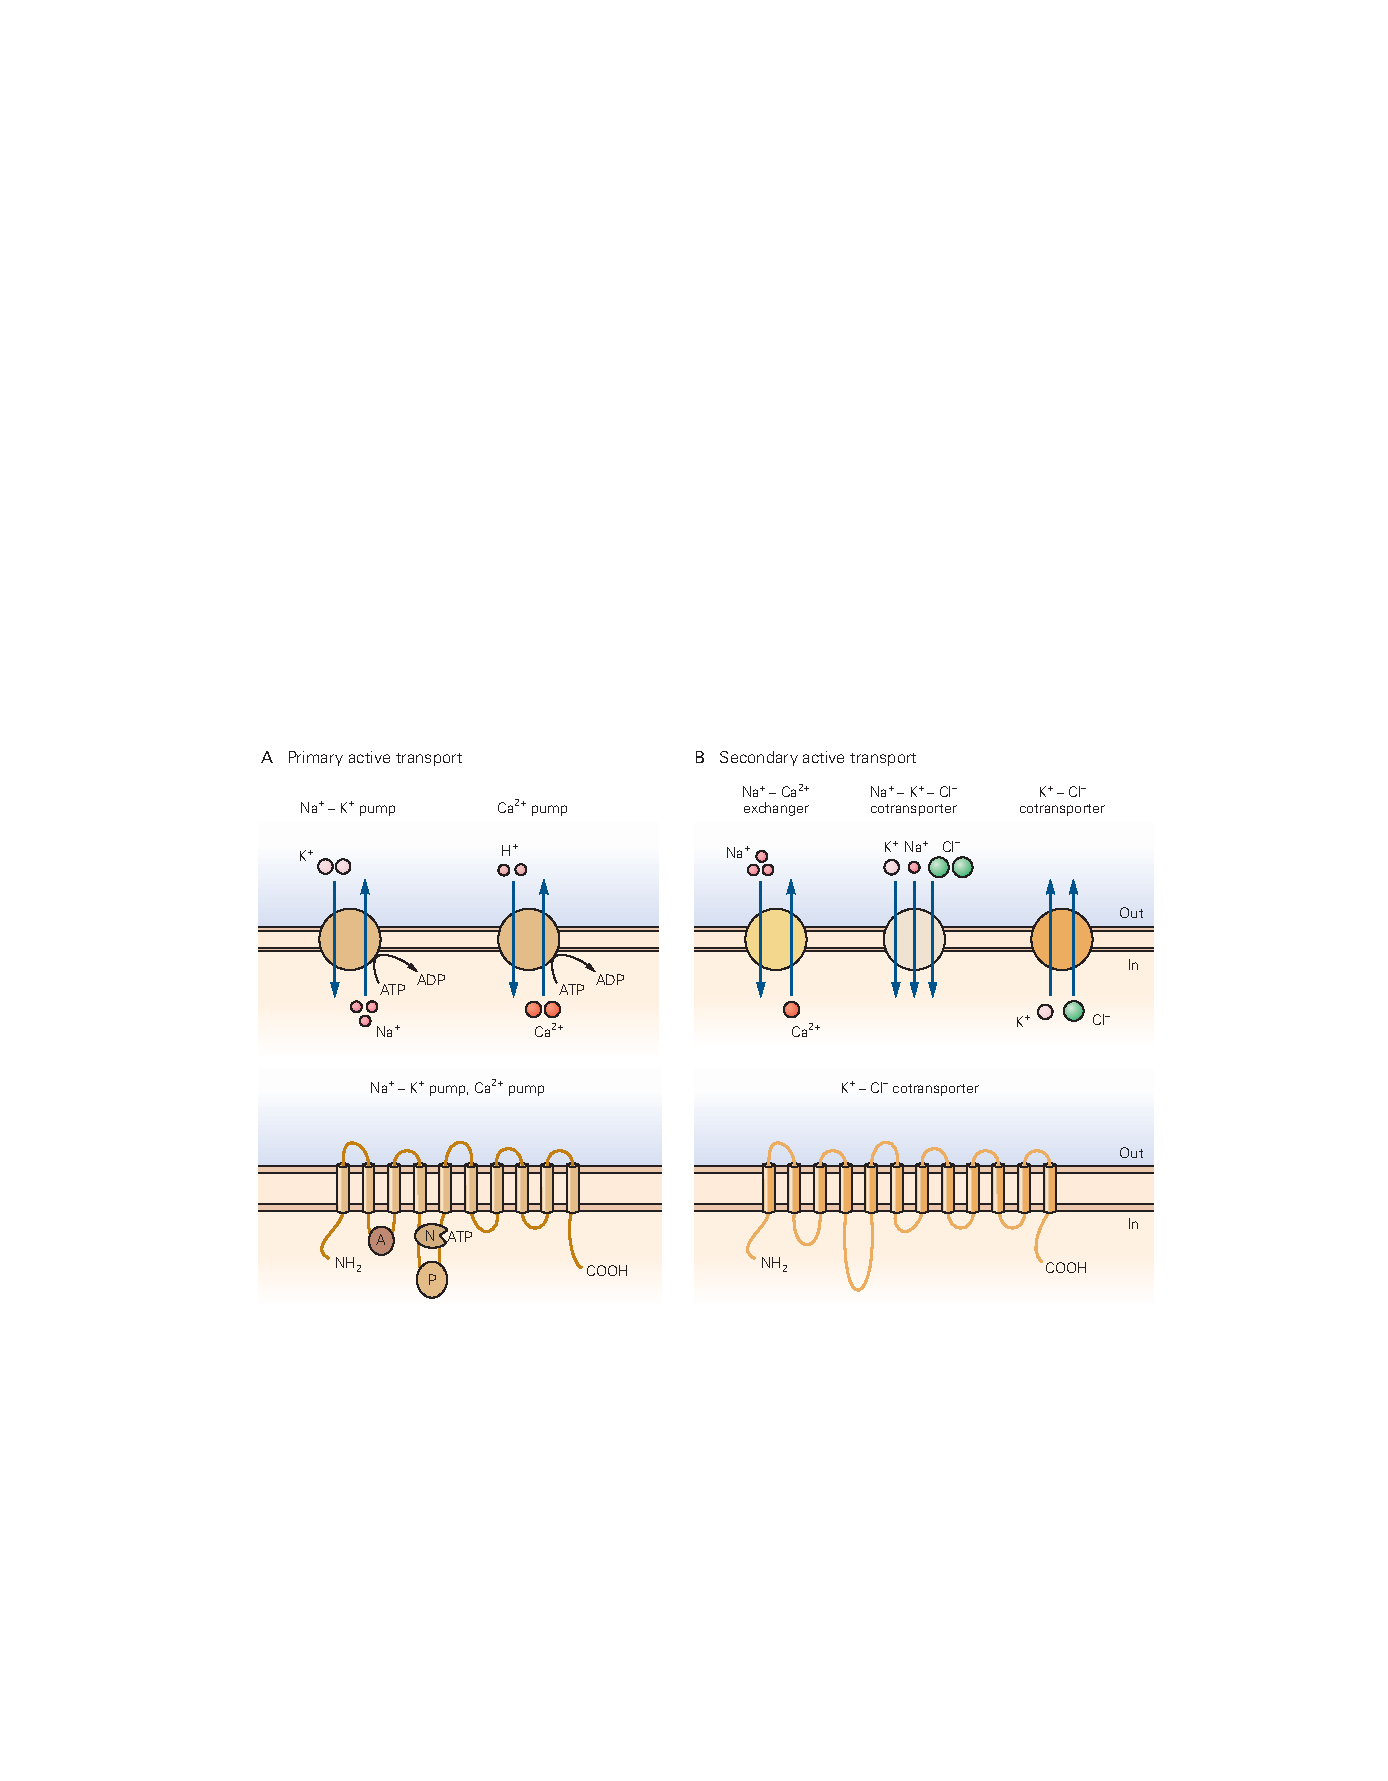
\includegraphics[width=0.7\linewidth]{chap09/fig_9_5}
	\caption{泵和转运蛋白调节 \ce{Na+}、\ce{K+}、\ce{Ca^2+} 和 \ce{Cl-} 离子的化学浓度梯度。 A. Na-\ce{K+} 泵和 \ce{Ca^2+} 泵是主动转运蛋白的两个例子,它们利用三磷酸腺苷 (ATP) 水解的能量来逆浓度梯度转运离子。 Na-\ce{K+} 泵或同源 Ca2+ 泵(下图)的 α 亚基具有 10 个跨膜区段、一个细胞质氨基末端和一个细胞质羧基末端。 还有一些细胞质环对于结合 ATP (N)、ATP 水解和磷酸化泵 (P) 以及将磷酸化转导至转运 (A) 很重要。 \ce{Na+}-\ce{K+} 泵还包含一个较小的 β 亚基,具有单个跨膜结构域和一个小的辅助整合膜蛋白 FXYD,它调节泵动力学(未显示)。 B. \ce{Na+}-\ce{Ca^2+} 交换器利用 \ce{Na+} 电化学梯度的势能将钙离子转运出细胞。 \ce{Na+}-钙离子交换器包含九个跨膜片段、两个对离子传输很重要的重入膜环和一个大的细胞质调节环。 氯离子通过 \ce{Na+}-\ce{K+}-\ce{Cl-} 协同转运蛋白转运到细胞内,并通过 \ce{K+}-\ce{Cl-} 协同转运蛋白转运出细胞。 这些转运蛋白是具有 12 个跨膜片段(下图)的 \ce{Cl-} 转运蛋白家族的成员。}
	\label{fig:9_5}
\end{figure}


\ce{Na+}-\ce{K+}泵和钙离子泵具有相似的结构。
它们由 110 kD α-亚基形成,其大跨膜结构域包含 10 个跨膜 α-螺旋(图~\ref{fig:9_5}A)。
在 \ce{Na+}-\ce{K+} 泵中,一个 α-亚基与一个必需的 β-亚基结合,后者是泵的正确组装和膜表达所必需的。
在人类中,四个基因编码高度相关的 \ce{Na+}-\ce{K+} 泵 α 亚基(ATP1A1、ATP1A2、ATP1A3、ATP1A4)。
ATP1A2 的突变会导致家族性偏瘫性偏头痛,这是一种与先兆和肌肉无力相关的偏头痛。
神经元特异性 ATP1A3 亚型中的某些突变会导致快速发作的肌张力障碍帕金森病,这是一种运动障碍,首先发生在青春期晚期或成年早期。
一组不同的突变会导致明显的神经系统疾病、儿童交替性偏瘫、影响身体一侧的瘫痪并在 2 岁以下的儿童中发生。


\ce{Na+}-\ce{K+}泵和钙离子泵具有相似的结构。
它们由 110 kD α-亚基形成,其大跨膜结构域包含 10 个跨膜 α-螺旋(图~\ref{fig:9_5} A)。
在 \ce{Na+}-\ce{K+} 泵中,一个 α-亚基与一个必需的 β-亚基结合,后者是泵的正确组装和膜表达所必需的。
在人类中,四个基因编码高度相关的 \ce{Na+}-\ce{K+} 泵 α 亚基(ATP1A1、ATP1A2、ATP1A3、ATP1A4)。 ATP1A2 的突变会导致家族性偏瘫性偏头痛,这是一种与先兆和肌肉无力相关的偏头痛。
神经元特异性 ATP1A3 亚型中的某些突变会导致快速发作的肌张力障碍帕金森病,这是一种运动障碍,首先发生在青春期晚期或成年早期。
一组不同的突变会导致明显的神经系统疾病、儿童交替性偏瘫、影响身体一侧的瘫痪并在 2 岁以下的儿童中发生。



\subsection{氯离子也被主动运输}
到目前为止,为简单起见,我们忽略了氯化物 (Cl−) 对静息电位的贡献。 
然而,在大多数神经细胞中,跨细胞膜的 \ce{Cl-} 梯度受一种或多种主动转运机制控制,因此 ECl 不同于 Vr。 
结果,开放的 \ce{Cl-} 通道的存在将使膜电位偏向其能斯特电位。 
氯离子转运蛋白通常使用存储在其他离子梯度中的能量——它们是协同转运蛋白。


细胞膜包含许多不同类型的 \ce{Cl-} 协同转运蛋白(图 \ref{fig:9_5} B)。 
一些转运蛋白将细胞内 \ce{Cl-} 增加到比 \ce{Cl-} 能斯特电位等于静息电位时被动达到的水平更高的水平。 
在此类细胞中,ECl 对 Vr 呈阳性,因此 \ce{Cl-} 通道的打开使膜去极化。 
这种类型的转运蛋白的一个例子是 \ce{Na+}-\ce{K+}-Cl− 协同转运蛋白。 
这种蛋白质将两个 \ce{Cl-} 离子与一个 \ce{Na+} 和一个 \ce{K+} 离子一起输送到细胞中。 
因此,转运体是电中性的。 
\ce{Na+}-\ce{K+}-Cl− 协同转运蛋白与 \ce{Na+}-钙离子交换剂的不同之处在于前者将所有三种离子沿同一方向转运——它是一种协同转运蛋白。


在大多数神经元中,\ce{Cl-} 梯度由将 \ce{Cl-} 移出细胞的协同转运蛋白决定。 
该作用降低了细胞内 \ce{Cl-} 的浓度,因此 ECl 通常比静息电位更负。 
结果,\ce{Cl-} 通道的打开导致 \ce{Cl-} 的流入,使膜超极化。 
\ce{K+}-\ce{Cl-} 协同转运蛋白就是这种转运机制的一个例子; 它每输出一个 \ce{Cl-} 离子,就会将一个 \ce{K+} 离子移出细胞。


有趣的是,在早期神经元发育过程中,细胞倾向于主要表达 \ce{Na+}-\ce{K+}-Cl− 协同转运蛋白。 
因此,在此阶段激活配体门控 \ce{Cl-} 通道的神经递质 γ-氨基丁酸 (GABA) 通常具有兴奋(去极化)作用。 
随着神经元的发育,它们开始表达 \ce{K+}-\ce{Cl-} 协同转运蛋白,因此在大多数成熟神经元中,GABA 通常会使膜超极化,从而充当抑制性神经递质。 
在成人的某些病理状况下,例如某些类型的癫痫或慢性疼痛综合征,\ce{Cl-} 协同转运蛋白的表达模式可能会恢复到未成熟神经系统的表达模式。 
这将导致对 GABA 的异常去极化反应,从而产生异常高水平的兴奋。



\section{静息膜中离子通量的平衡在动作电位期间被取消}

在静止的神经细胞中,稳定的 \ce{Na+} 流入被稳定的 \ce{K+} 流出所平衡,因此膜电位是恒定的。 
当膜朝着动作电位的阈值去极化时,这种平衡会发生变化。 
当膜电位接近该阈值时,电压门控 \ce{Na+} 通道迅速打开。 
一旦超过阈值,膜对 \ce{Na+} 电导的增加导致 \ce{Na+} 流入超过 \ce{K+} 流出,产生正电荷净流入,导致进一步去极化。 
去极化的增加导致更多的电压门控 \ce{Na+} 通道打开,导致更多的 \ce{Na+} 流入,从而进一步加速去极化。


这种再生的正反馈循环呈爆炸式发展,将膜电位快速推向 +55 mV 的 \ce{Na+} 平衡电位:

然而,膜电位永远不会完全达到 ENa,因为 \ce{K+} 流出在整个去极化过程中持续进行。 
少量 Cl− 流入细胞也会抵消 \ce{Na+} 流入的去极化作用。 
然而,在动作电位的上升阶段,许多电压门控 \ce{Na+} 通道打开,以至于细胞膜的 \ce{Na+} 电导远大于 \ce{Cl-} 或 \ce{K+} 的电导。 
因此,在动作电位的峰值处,膜电位接近 \ce{Na+} 平衡电位,就像在静止时(当对 \ce{K+} 的渗透性占主导地位时)一样,膜电位趋于接近 \ce{K+} 平衡电位。


\section{不同离子对静息膜电位的贡献可以通过 Goldman 方程量化}
尽管 \ce{K+}、\ce{Na+} 和 Cl− 通量设定了静息电位值,但 Vm 不等于 EK、ENa 或 ECl,而是处于某个中间值。 
作为一般规则,当 Vm 由两种或多种离子决定时,一种物质的贡献不仅取决于细胞内外的离子浓度,还取决于离子穿过膜的难易程度。


衡量离子穿过膜的容易程度的一种方便的测量方法是膜对该离子的渗透率 (P),其单位是速度 (cm/s)。 
该度量类似于扩散常数的度量,它决定了由局部浓度梯度驱动的溶液中溶质运动的速率。 
膜电位对离子渗透性和浓度的依赖性由 Goldman 方程给出:


该等式仅在 Vm 不变时适用。 
它指出离子种类的浓度越大,其膜渗透性越大,其对确定膜电位的贡献就越大。 
在极限情况下,当对一种离子的渗透性异常高时,Goldman 方程简化为该离子的 Nernst 方程。 
例如,如果 PK >> PCl 或 PNa,如在神经胶质细胞中,方程变为如下:


Alan Hodgkin 和 Bernard Katz 使用 Goldman 方程分析了乌贼巨型轴突中膜电位的变化。 
他们测量了膜电位的变化以响应细胞外 \ce{Na+}、\ce{Cl-} 和 \ce{K+} 浓度的系统变化。 
他们发现,如果在细胞外浓度改变后不久(在内部离子浓度改变之前)测量 Vm,[\ce{K+}]o 对静息电位有很强的影响,[Cl−]o 有中等影响,[\ce{Na+}] ]o 影响不大。 
静止膜的数据可以使用以下渗透率比率通过 Goldman 方程准确拟合:


在动作电位的峰值处,有一个瞬间 Vm 没有变化,Goldman 方程适用。 
在这一点上,如果假设一组完全不同的渗透率比,则 Vm 随外部离子浓度的变化最合适:


对于这些渗透率值,Goldman 方程接近于 \ce{Na+} 的 Nernst 方程:


因此,在动作电位的峰值处,当膜对 \ce{Na+} 的渗透性远高于对任何其他离子的渗透性时,Vm 接近 ENa。 
然而,膜对 \ce{K+} 和 \ce{Cl-} 的有限渗透性导致 \ce{K+} 流出和 \ce{Cl-} 流入,部分抵消了 \ce{Na+} 流入,从而阻止 Vm 完全达到 ENa。



\section{神经元的功能特性可以表示为等效回路}

Goldman 方程的实用性是有限的,因为它不能用于确定膜电位如何随时间或神经元内的距离变化以响应局部渗透性变化。
也不方便确定单个 \ce{Na+}、\ce{K+} 和 Cl− 电流的大小。
可以使用源自回路理论的简单数学模型获得此信息。
该模型称为等效回路,通过由导体或电阻器、电池和电容器组成的回路表示神经元的所有重要电气特性。
等效回路为我们提供了直观的理解以及离子运动引起的电流如何在神经细胞中产生电信号的定量描述。


开发等效回路的第一步是将膜的离散物理特性与其电特性联系起来。
脂质双层赋予膜电容,即非导体(绝缘体)分离膜两侧电荷的能力。
膜的非导电磷脂双分子层将细胞质和细胞外液分开,两者都是高度导电的环境。
细胞膜(电容器)内外表面的电荷分离导致跨膜的电势差。
电容器两端的电势差或电压为:
\begin{equation}
	V = Q/C,
\end{equation}
其中 Q 是电容器每一侧的净过量正电荷或负电荷,C 是电容。


电容以法拉 (F) 为单位测量,电荷以库仑测量(其中 96,500 库仑的一价离子相当于 1 摩尔该离子)。
1 F 电容器上 1 库仑的电荷分离会产生 1 伏特的电势差。
神经细胞的典型膜电容值约为每平方厘米膜面积 1 μF。 
需要很少的电荷就可以在这种电容上产生显着的电位差。 
例如,直径为50 μm、静息电位为-60 mV的球形细胞体的膜隔开的正负电荷过剩为29×106个离子。
尽管这个数字看起来很大,但它仅代表细胞质内溶液中正电荷或负电荷总数的一小部分 (1/200,000)。
大部分细胞质和大部分细胞外液是电中性的。


该膜是一个漏电电容器,因为它布满了可以传导电荷的离子通道。
离子通道赋予膜电导和产生电位差的能力。
脂质双层本身实际上具有零电导或无穷大电阻。
然而,由于离子通道具有高导电性,它们为离子穿过膜提供了有限电阻的途径。
因为神经元包含许多类型的通道,对不同的离子具有选择性,我们必须分别考虑每一类离子通道。


在等效回路中,我们可以将每个 \ce{K+} 通道表示为具有单通道电导 γK 的电阻器或离子电流导体(记住,电导 = 1/电阻)(图~\ref{fig:9_6}A)。 
如果没有 \ce{K+} 浓度梯度,通过单个 \ce{K+} 通道的电流将由欧姆定律给出:iK = γK × Vm。
然而,通常存在 \ce{K+} 浓度梯度,因此也存在驱动 \ce{K+} 跨膜的化学力,在等效回路中由电池表示。
(电势源称为电动势 [EMF],由化学势差产生的电动势称为电池。)该电池的电动势由 EK 给出,即 \ce{K+} 的能斯特电势(图~\ref{fig:9_6})。


\begin{figure}[htbp]
	\centering
	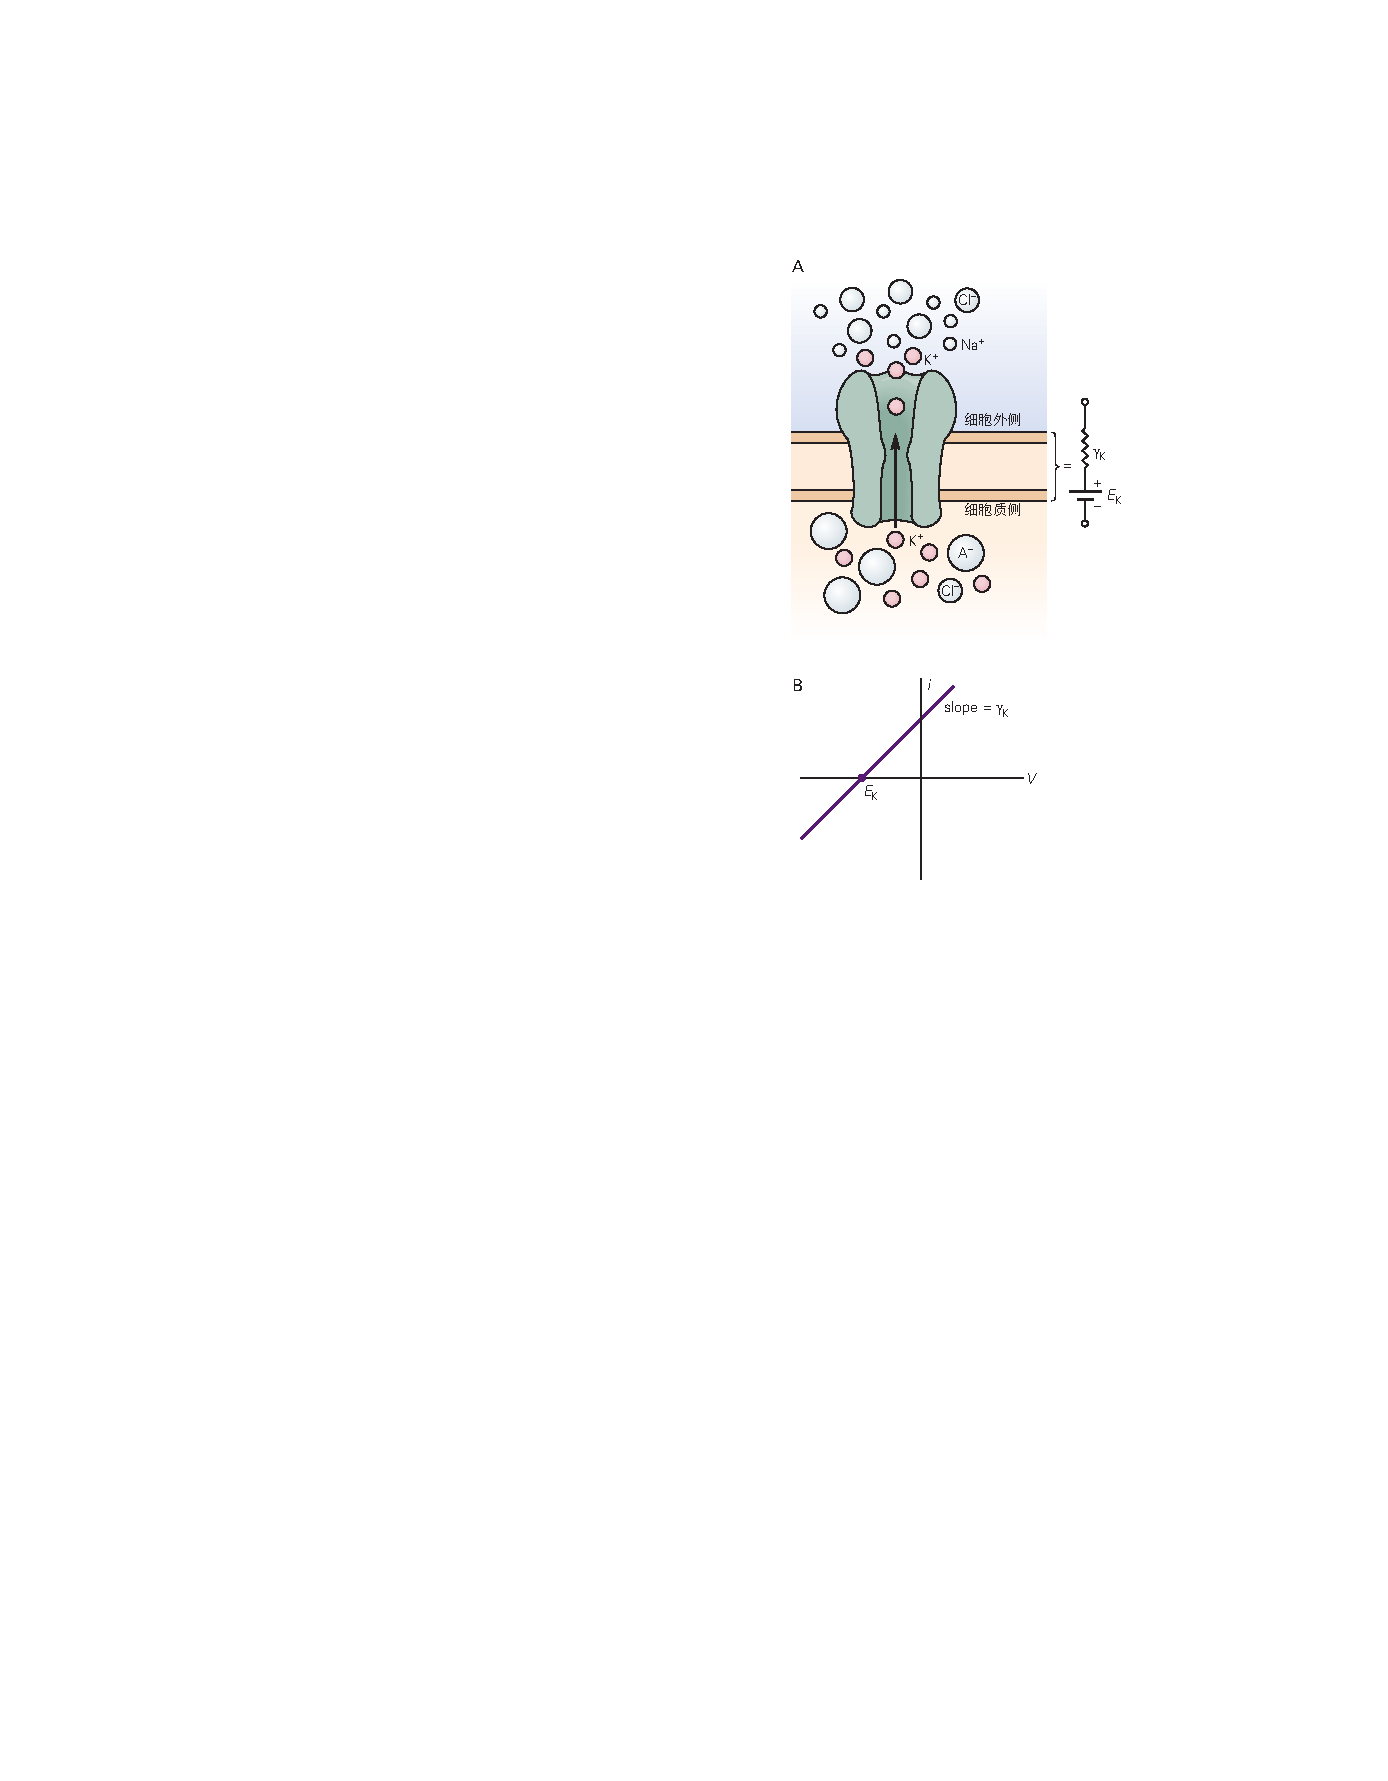
\includegraphics[width=0.5\linewidth]{chap09/fig_9_6}
	\caption{化学力和电力有助于电流通过离子通道。 A. \ce{K+} 的浓度梯度会产生电动势,其值等于 EK,即 \ce{K+} 的能斯特电势。 这可以用电池来表示。 在该回路中,电池EK与导体γK串联,代表\ce{K+}通道的电导。 B. 在电驱动力和化学驱动力同时存在的情况下,\ce{K+} 通道的电流-电压关系。 电流为零时的膜电位等于 \ce{K+} 能斯特电位。}
	\label{fig:9_6}
\end{figure}


在跨膜电压不存在的情况下,正常的 \ce{K+} 浓度梯度会导致向外的 \ce{K+} 电流。
根据我们对电流的约定,正电荷跨膜向外移动对应于正电流。
根据 Nernst 方程,当带正电的离子(例如 \ce{K+})的浓度梯度向外(即细胞内的 \ce{K+} 浓度高于细胞外)时,该离子的平衡电位为负。
因此,仅由于其浓度梯度而流动的 \ce{K+} 电流由 iK = −γK × EK 给出(负号是必需的,因为负平衡电位在 0 mV 时产生正电流)。


最后,对于同时具有膜电位和 \ce{K+} 浓度梯度的真实神经元,净 \ce{K+} 电流由电驱动力和化学驱动力引起的电流之和给出:


因子 (Vm − EK) 称为电化学驱动力。
它决定了离子电流的方向和(连同电导)它的大小。
该方程式是欧姆定律的一种修改形式,它考虑了这样一个事实,即通过膜的离子电流不仅取决于跨膜电压,还取决于离子浓度梯度。


细胞膜有许多静止的 \ce{K+} 通道,所有这些通道都可以组合成一个由与电池串联的导体组成的等效回路元件。
在这个等效回路中,所有 \ce{K+} 通道的总电导 (gK),即细胞膜在静息状态下的 \ce{K+} 电导,等于静息 \ce{K+} 通道数 (NK) 乘以个体的电导 \ce{K+}通道(γK):


由于此等效回路中的电池仅取决于 \ce{K+} 的浓度梯度,而与 \ce{K+} 通道的数量无关,因此其值为 \ce{K+} 的平衡电位 EK。


与静息 \ce{K+} 通道群一样,所有静息 \ce{Na+} 通道都可以由与单个电池串联的单个导体表示,静息 \ce{Cl-} 通道也是如此。
由于 \ce{K+}、\ce{Na+} 和 Cl− 通道占静止细胞中通过细胞膜的大部分被动离子电流,我们可以通过将这三种途径合并到神经元的简单等效回路中来计算静息电位(图 9–7)。


为了完成这个回路,我们首先将代表每种类型通道的元素与代表细胞外液和细胞质的元素连接起来。
细胞外液和细胞质都是良导体(与细胞膜相比),因为它们具有相对较大的横截面积和许多可携带电荷的离子。
在神经元的一个小区域中,细胞外和细胞质电阻可以近似为短路——零电阻导体。
膜电容 (Cm) 由脂质双层的绝缘特性及其面积决定。


最后,可以通过结合由 \ce{Na+}-\ce{K+} 泵驱动的活性离子通量来完成等效回路,该泵每泵入两个 \ce{K+} 离子,就会从细胞中挤出三个 \ce{Na+} 离子。
这种生电 ATP 依赖泵,可以保持充电的离子电池,在等效回路中用电流发生器的符号表示(图~\ref{fig:9_7} )。
方框~\ref{box:9_2}~说明了使用等效回路定量分析神经元特性,其中等效电路用于计算静息电位。


\begin{proposition}[利用等效电路模型计算静息膜电位] \label{box:9_2}
	
	\quad \quad 静息膜的等效电路模型可用于计算静息电位(图9-8)。
	为了简化计算,我们忽略了\ce{Na+}-\ce{K+}泵的产电影响,因为它很小。
	我们也忽略了膜电容,因为Vm不变,所以电容上的电荷也没有变化。
	
	\quad \quad 由于\ce{K+}的静息通道比\ce{Na+}的静息通道多,因此\ce{K+}的膜电导远大于\ce{Na+}的膜电导。在图9-8的等效电路中,gK(10×10-6 S)比gNa(0.5×10-6 S)高20倍。
	对于大多数神经细胞,gCl的值范围为gK的四分之一到一半。
	在这个例子中,gCl等于4.0×10-6 S。给定这些值以及EK,ECl和ENa的值,我们可以如下计算Vm。
	
	\quad \quad 由于膜电位是恒定的,因此通过三组离子通道没有净电流:
	
	\quad \quad 我们可以很容易地分两步计算每个电流。
	首先,我们将电路每个分支上的单独电位差相加。
	例如,在\ce{K+}分支中,总电位差是电池EK和欧姆定律给出的跨越gK的压降之和(Vm=IK/gK):*
	
	\quad \quad 同样,对于\ce{Na+}和\ce{Cl-}电导分支:
	
	\quad \quad 接下来,我们重新排列并求解每个分支中的离子电流I:
	
	\quad \quad 这些方程类似于方程9-1,其中通过单个离子通道的净电流来自各个驱动力产生的电流。
	如这些方程所示,通过每个电导分支的离子电流等于该分支的电导乘以净电化学驱动力。
	因此,对于\ce{K+}电流,电导与开放\ce{K+}通道的数量成正比,驱动力等于Vm和EK之间的差值。
	如果Vm比EK(-75 mV)更正,则驱动力为正,电流为向外;
	如果Vm比EK更负,则驱动力为负,电流向内。
	
	\quad \quad 在本书中,类似的方程被用于各种情况,以将特定离子电流的大小与其膜电导和驱动力联系起来。
	
	\quad \quad 正如我们在等式9-2中所看到的,I\ce{Na+}I\ce{K+}ICl=0。
	如果我们现在用等式9-3a,b,c代替等式9-2中的INa,IK和ICl,乘以并重新排列,我们得到以下表达式:
	
	\quad \quad 求解Vm,我们得到了静息膜电位的方程,该方程用膜电导g和电池E表示:
	
	\quad \quad 从这个方程中,使用等效电路中的值(图9-8),我们计算出Vm=-70 mV。
	
	\quad \quad 等式9-4表明Vm接近电导较大的离子电池的值。
	这个原理可以通过考虑动作电位期间发生的事情来说明。
	在动作电位的峰值,gK和gCl与静息值基本不变,但gNa增加了500倍。
	gNa的这种增加是由电压门控\ce{Na+}通道的开放引起的。
	在图9-8中的等效电路中,增加500倍将使gNa从0.5×10-6 S变为250×10-6 S。
	
	\quad \quad 如果我们将gNa的这个新值替换为等式9-4并求解Vm,则得到+48 mV。
	在动作电位的峰值处,Vm比EK更接近ENa,因为gNa现在比gK大25倍,比gCl大62.5倍,因此在确定Vm时,\ce{Na+}电池比\ce{K+}和\ce{Cl-}电池重要得多。
	
	\quad \quad 方程9-4类似于Goldman方程,因为每个离子电池对Vm的贡献与该特定离子的膜电导成比例加权。
	在极限范围内,如果一个离子的电导远大于其他离子的电导,则Vm接近该离子的能斯特势值。
	
	\quad \quad 通过将所有有助于静息电位的静息通道的电导集中为单个电导gr,并用单个电池Er替换每个电导通道的电池,可以进一步简化等效电路,其值由等式9-4给出(图9-9)。
	这里的下标r代表静息通道途径。由于静息通道为离子在膜上的稳定泄漏提供了途径,因此它们有时被称为泄漏通道(第~\ref{chap:chap10}~章)。
	当我们在后面的章节中考虑通过电压门控和配体门控通道的电流对膜电压的影响时,这种静息途径的巩固将证明是有用的。
	
\end{proposition}



\begin{figure}[htbp]
	\centering
	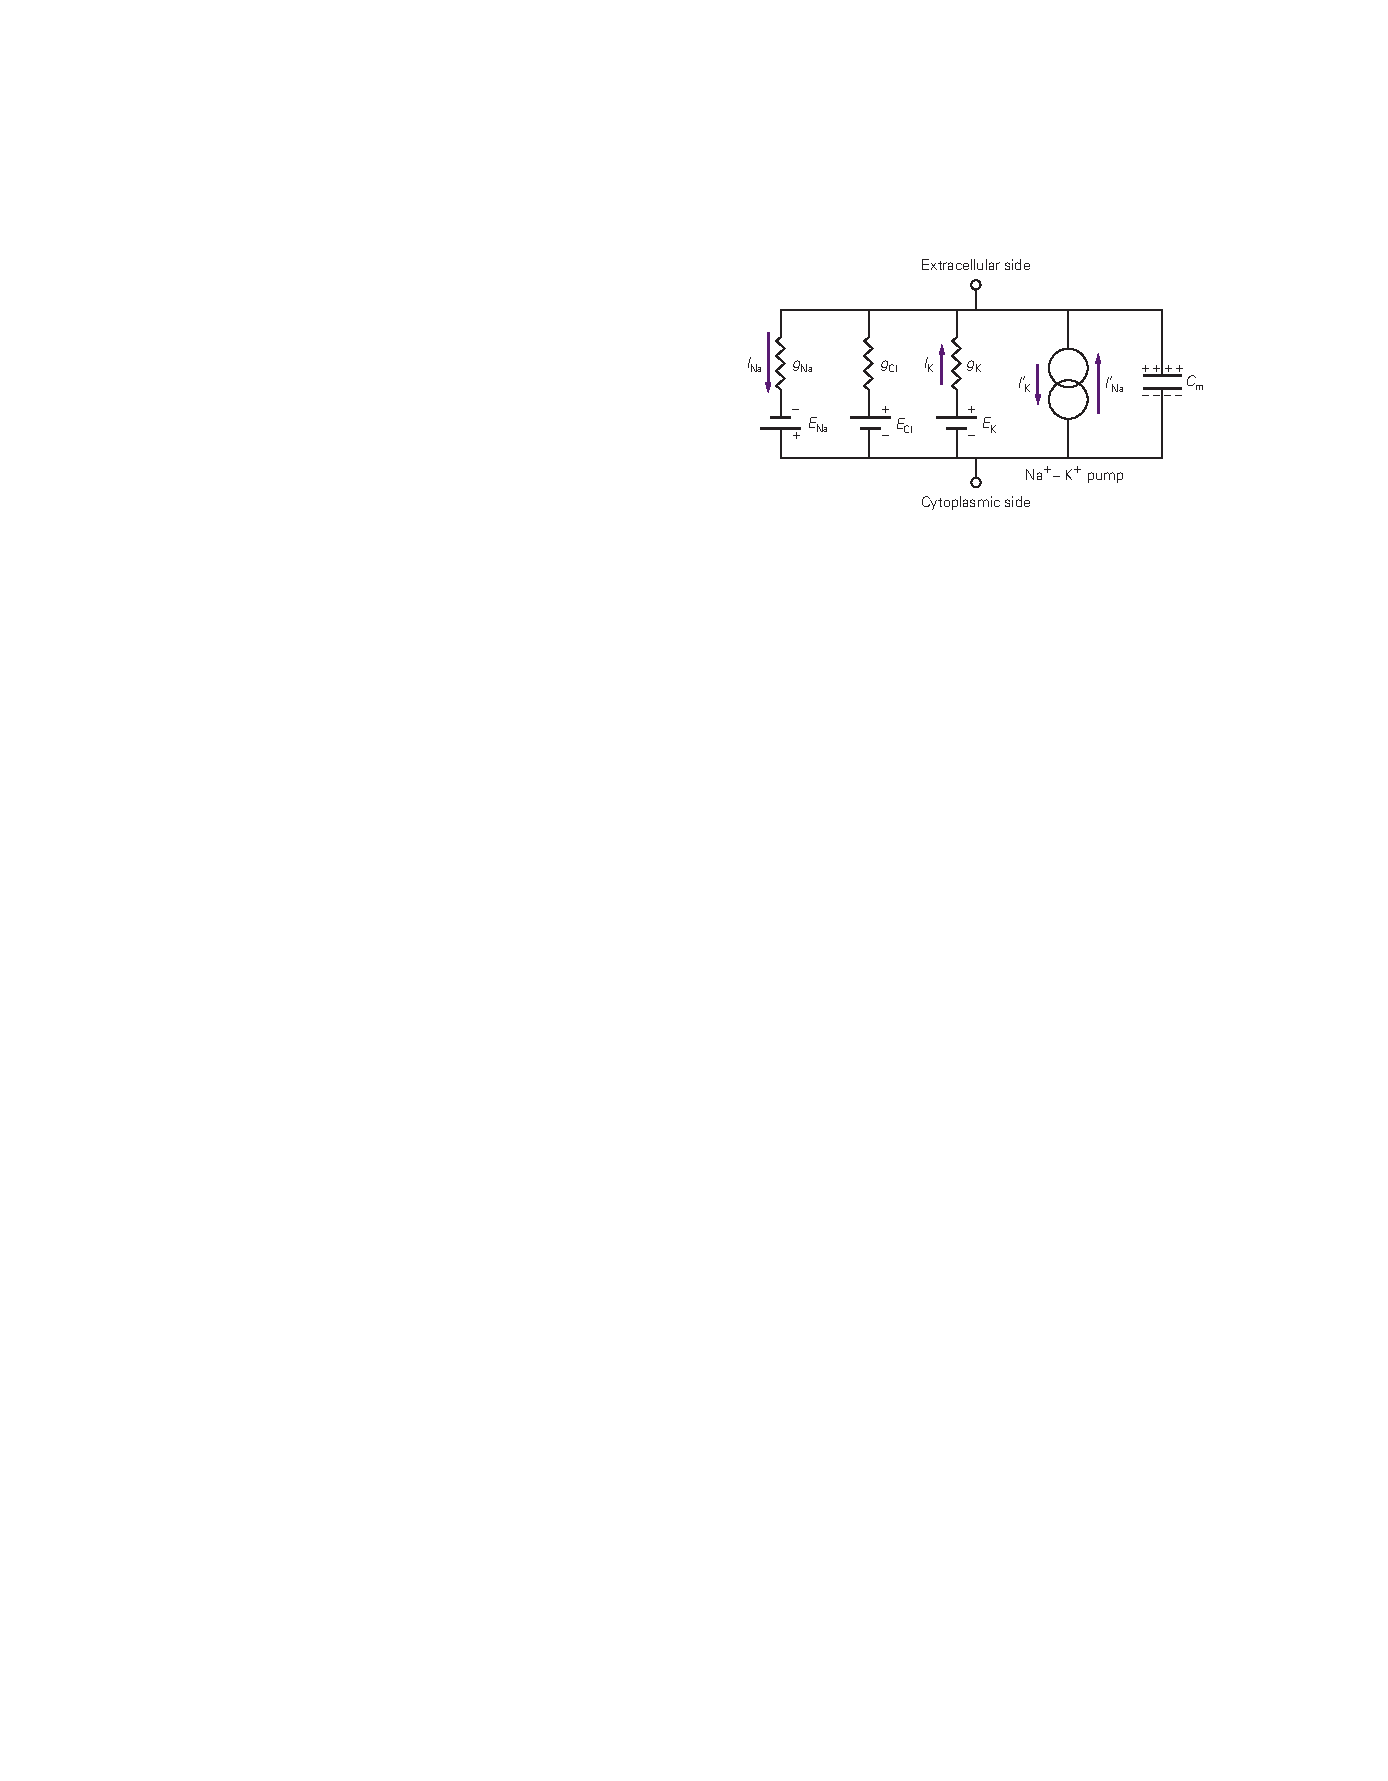
\includegraphics[width=0.5\linewidth]{chap09/fig_9_7}
	\caption{静息神经元中被动电流和主动电流的等效回路。 由符号 gK 表示的总 \ce{K+} 电导是 γK × N(静息膜中开放的 \ce{K+} 通道总数)的乘积。 \ce{Na+} 和 \ce{Cl-} 通道的总电导以类似的方式确定。 在稳态条件下,被动 \ce{Na+} 和 \ce{K+} 电流由 Na-\ce{K+} 泵驱动的主动 \ce{Na+} 和 \ce{K+} 通量(I 'Na 和 I 'K)平衡。 活性 \ce{Na+} 通量 (I ′Na) 比活性 \ce{K+} 通量 (I ′K) 高 50\%,因为 \ce{Na+}-\ce{K+} 泵每向细胞输送两个 \ce{K+} 离子,就会输送三个 \ce{Na+} 离子。 因此,要使电池保持稳定状态,INa 必须比 IK 大 50\%(箭头大小与电流大小成正比)。 没有电流通过 Cl− 通道,因为在此示例中 Vm 处于 ECl,即 Cl− 平衡电位。}
	\label{fig:9_7}
\end{figure}


\section{神经元的被动电特性影响电信号}

一旦神经元的一部分产生电信号,例如响应树突分支上的突触输入,它就会与神经元的其他输入整合,然后传播到轴突起始段,即作用部位 潜在的一代。
当神经元中产生突触电位、受体电位或动作电位时,膜电位会迅速变化。


什么决定了电势随时间或距离的变化率?
是什么决定了刺激是否会产生动作电位?
在这里,我们考虑神经元的被动电特性和几何形状,以及这些相对恒定的特性如何影响细胞的电信号。 
门控通道的作用和改变膜电位的离子流将在接下来的五章中描述。


神经元具有三种对电信号传输很重要的被动电特性。 
我们已经描述了静息膜电导或电阻 (gr = 1/Rr) 和膜电容 Cm。 
决定信号沿树突或轴突传播的第三个重要特性是它们的细胞内轴向阻力 (ra)。 
尽管细胞质的电阻率远低于细胞膜的电阻率,但沿延伸的薄神经元过程的整个长度的轴向阻力可能相当大。 
由于这三个元素提供了在活性离子电流流入或流出细胞时完成回路的返回路径,因此它们决定了突触电流产生的突触电位变化的时间进程。 
他们还确定树突中产生的突触电位是否会使轴突初始段的触发区去极化,足以激发动作电位。 
最后,被动属性影响动作电位传导的速度。


\subsection{薄膜电容减缓了电信号的时程}
响应亚阈值电流的神经元电压的稳态变化类似于简单电阻器的行为,但变化的时间过程并非如此。 
真正的电阻器会以类似的电压阶跃变化响应电流阶跃变化,但由于其电容,神经元的膜电位上升和衰减比电流阶跃变化更慢(图 \ref{fig:9_10})。

\begin{figure}[htbp]
	\centering
	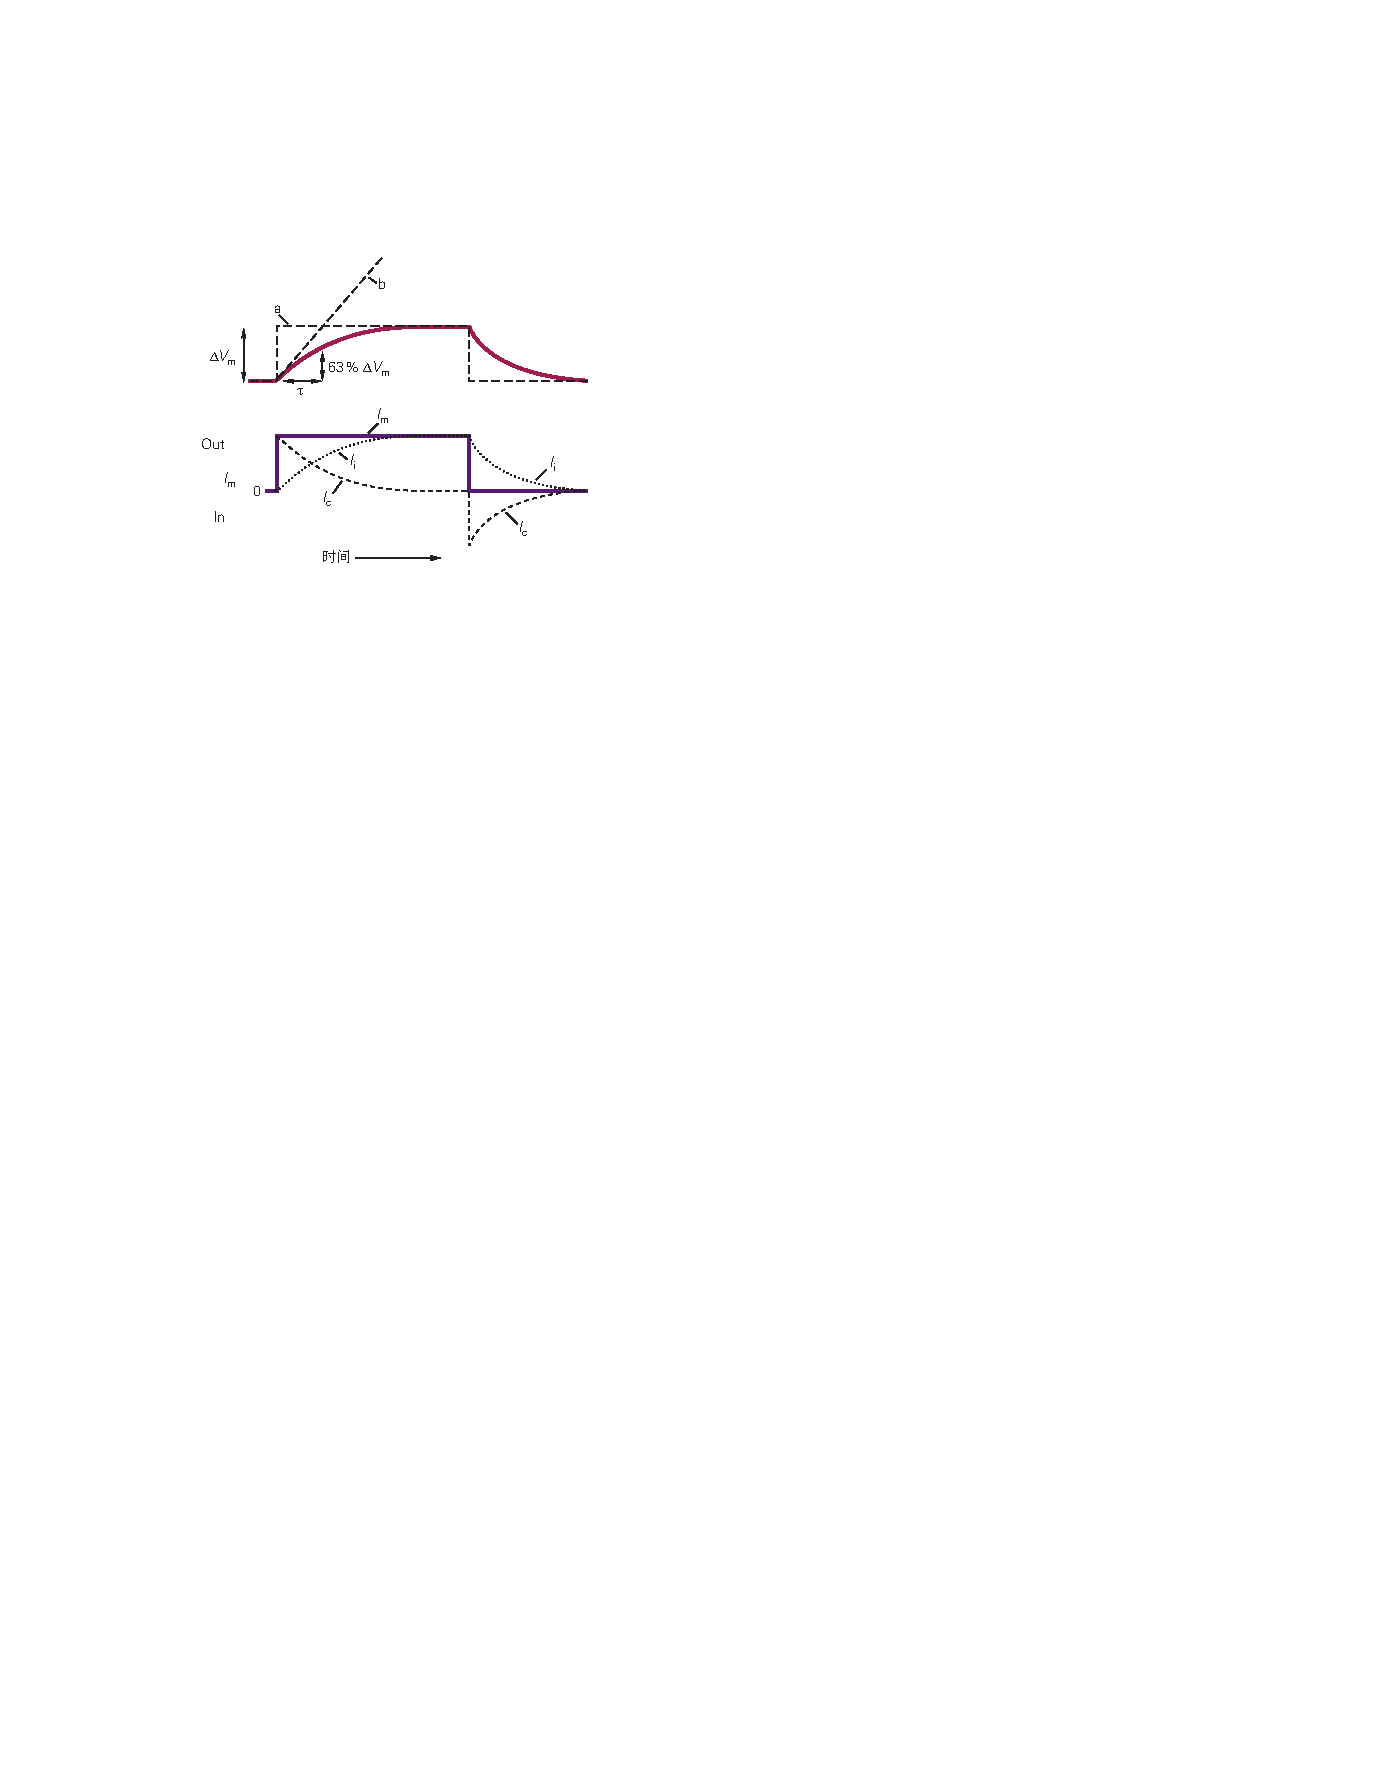
\includegraphics[width=0.5\linewidth]{chap09/fig_9_10}
	\caption{膜电位的变化率因膜电容而减慢。 上图显示了膜电位 (ΔVm) 对阶跃电流脉冲 (Im) 的响应。 实际电压响应的形状(红线)结合了纯电阻元件(虚线 a)和纯电容元件(虚线 b)的特性。 达到最终电压的 63\% 所需的时间定义了膜时间常数 τ。 下图显示了电流脉冲期间总膜电流 (Im) 的两个元素:跨膜电阻元件(离子通道)的离子电流 (Ii) 和电容电流 (Ic)。}
	\label{fig:9_10}
\end{figure}


要了解电容如何减慢电压响应,请回想一下电容器两端的电压与电容器上存储的电荷成正比。 
要改变电压,电荷 Q 必须添加到电容器 C 或从电容器 C 中移除:


要改变电容器(膜脂双层)上的电荷,电容器 (Ic) 上必须有电流。 
由于电流是每单位时间的电荷流量 (Ic = ΔQ/Δt),因此电容器两端的电压变化是电流大小和持续时间的函数:


因此,电容器两端的电压响应电流脉冲的变化幅度取决于电流的持续时间,因为需要时间来从电容器沉积和移除电荷。


如果膜仅具有电阻特性,则向外电流的阶跃脉冲会立即改变膜电位。 
相反,如果膜仅具有电容特性,则膜电位将响应相同的电流阶跃随时间线性变化。 
由于膜同时具有电容和电阻特性,因此膜电位的实际变化结合了两种纯响应的特征。 
变化的初始斜率反映了纯电容元件,而最终斜率和幅度反映了纯电阻元件(图 \ref{fig:9_10},上图)。


在神经元的球形细胞体的简单情况下,电势变化的时间过程由以下等式描述:


其中 e 是自然对数系统的底数,其值约为 2.72,τ 是膜时间常数,由膜电阻和电容 (RmCm) 的乘积给出。
时间常数可以通过实验测量,因为膜电位上升到 1 − 1/e 或大约其稳态值的 63\% 所需的时间(图 \ref{fig:9_10},上图)。 
神经元 τ 的典型值范围为 20 到 50 毫秒。 我们将回到第~\ref{chap:chap13}~章中的时间常数,在那里我们考虑细胞中突触输入的时间总和。



\subsection{膜和细胞质电阻影响信号传导的效率}

到目前为止,我们已经考虑了神经元的被动特性仅对细胞体内信号传导的影响。
距离不是神经元胞体中信号传播的一个因素,因为细胞体可以近似为一个球体,其膜电压是均匀的。
然而,沿着扩展结构(树突、轴突和肌纤维)传播的亚阈值电压信号的振幅随着距起始点的距离的增加而减小,因为一些电荷在沿着树突或轴突流动时从静息膜电导中泄漏。
为了说明这种衰减是如何发生的,我们将考虑神经元的几何形状如何影响电流的分布。


\begin{figure}[htbp]
	\centering
	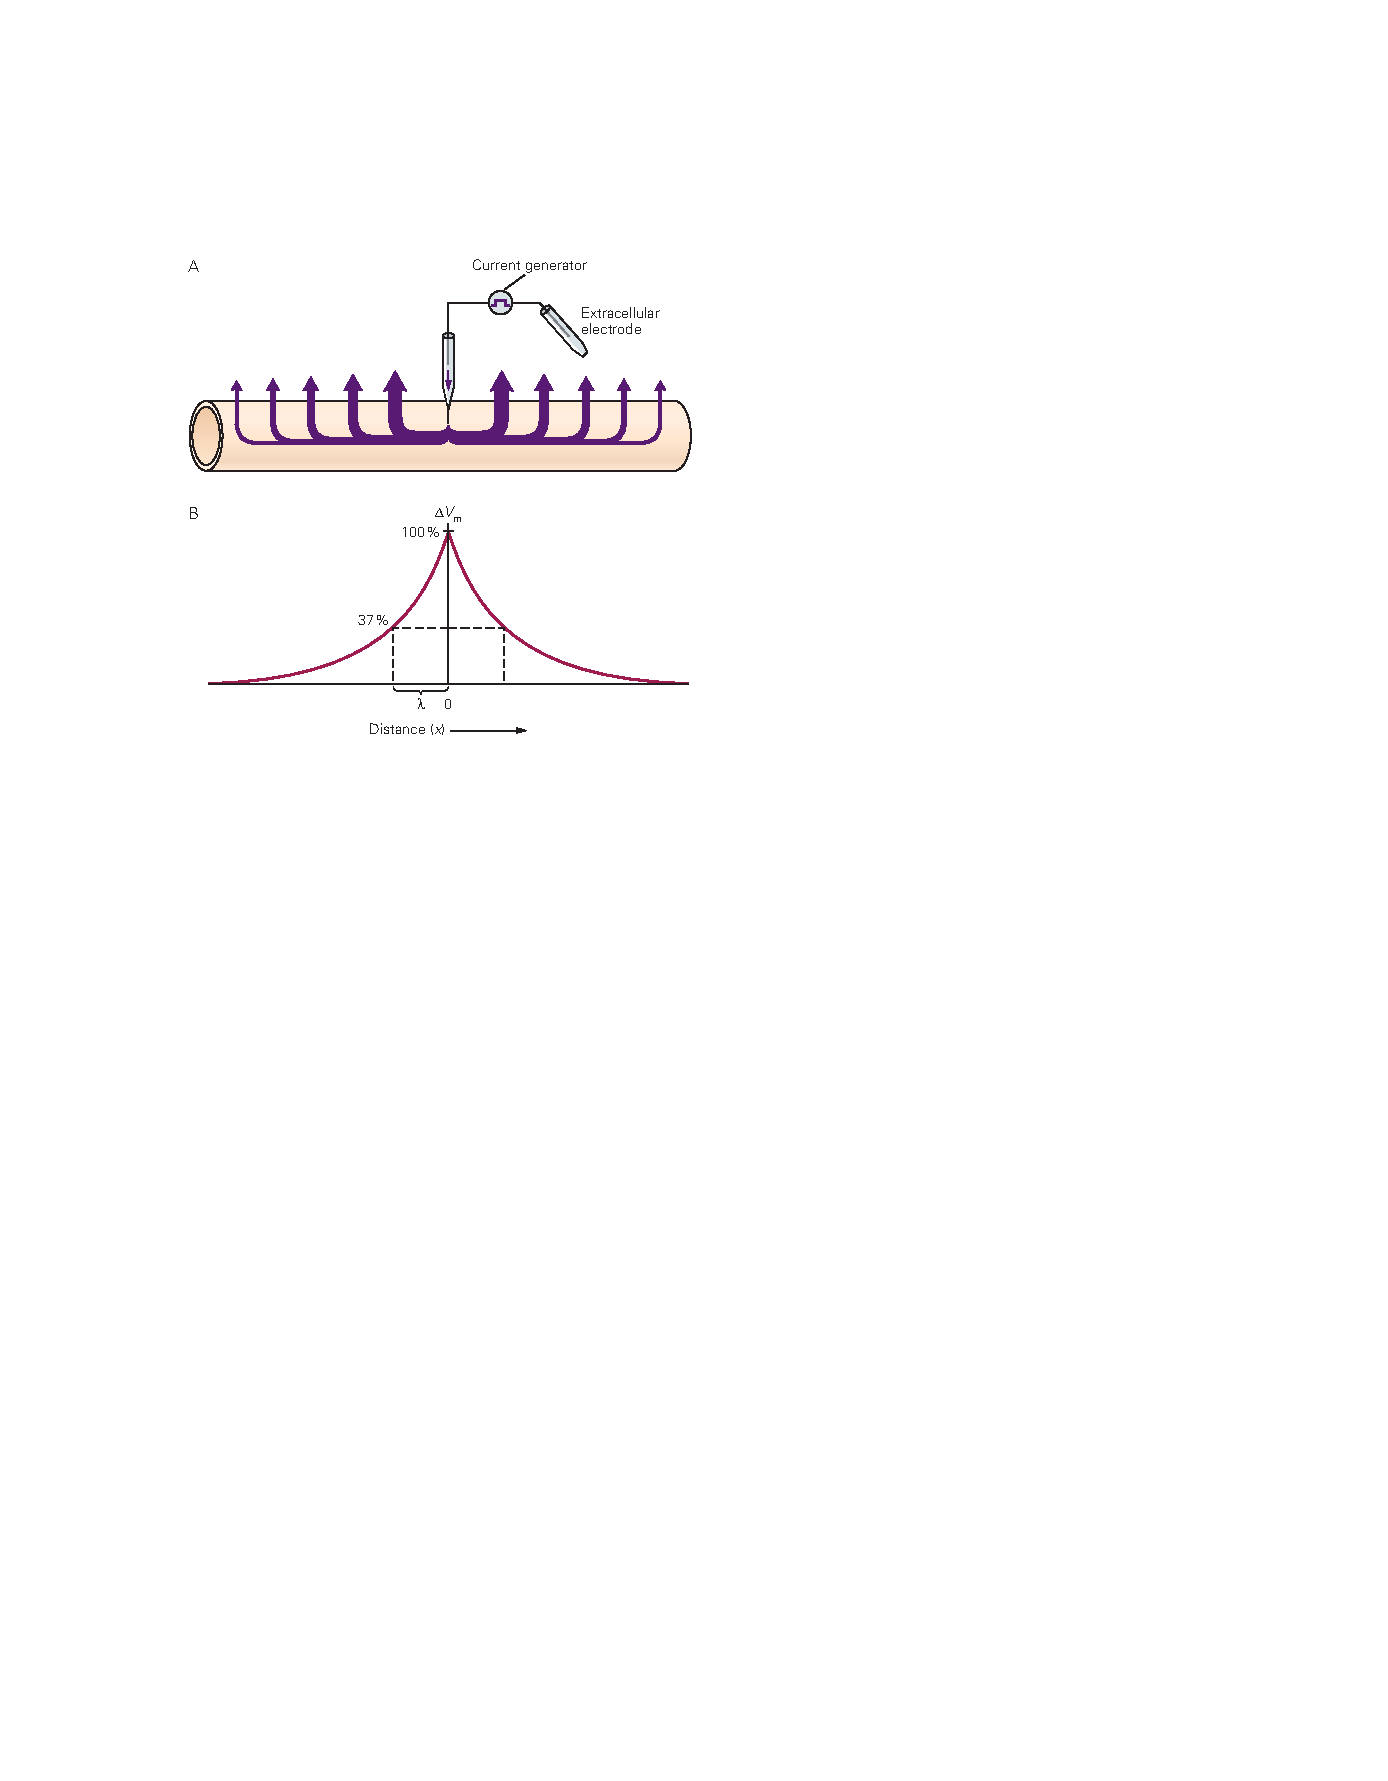
\includegraphics[width=0.5\linewidth]{chap09/fig_9_11}
	\caption{电紧张传导过程中神经元过程中膜电位的变化随距离的增加而减小。 A. 通过微电极注入神经元过程的电流遵循细胞外液中返回电极的阻力最小的路径。 (箭头的粗细表示膜电流的大小。) B. Vm 的变化随着距电流注入点的距离呈指数衰减。 ΔVm 衰减到电流注入点值的 37\% 时的距离定义了长度常数 λ。}
	\label{fig:9_11}
\end{figure}


如果电流在某一点注入树突,膜电位将如何沿其长度变化?
为简单起见,考虑在恒幅电流脉冲持续一段时间 (t >> τ) 后膜电位如何随距离变化。
在这些条件下,膜电容充满电,因此膜电位达到稳定值。 电势随距离的变化取决于从树突中泄漏的电荷与在树突内流向胞体的电荷的比例。
由于电荷沿着阻力最小的路径流动,这取决于单位长度枝晶的膜电阻rm(单位为Ω·cm)和单位长度枝晶的轴向电阻ra(单位为Ω/cm)的相对值 )。
沿树突的膜电位变化随着与电流电极的距离的增加而变小(图~\ref{fig:9_11} A)。
这种随距离的衰减是指数的,表示为


其中 λ 是膜长度常数,x 是距电流注入点的距离,ΔV0 是电流在注入点 (x = 0) 处产生的膜电位变化。 
长度常数是沿着枝晶到 ΔVm 衰减到 1/e 或其初始值的 37\% 的位置的距离(图 9–11B)。
它是电紧张传导效率的量度——电压变化沿神经元的被动扩散——由膜电阻和轴向电阻的值决定,如下所示:


膜的绝缘性越好(即 rm 越大)和内核的导电性能越好(ra 越低),枝晶的长度常数越大。
这是因为电流能够沿着树突的内部导电核心扩散得更远,然后在某个点 x 处泄漏穿过膜以改变局部膜电位:


长度常数也是神经元突直径的函数。
神经元突起的直径差异很大,从乌贼巨型轴突的 1 毫米到哺乳动物大脑中细树突分支的 1 微米不等。
对于具有相似离子通道表面密度(每单位膜面积的通道数)和细胞质组成的神经元过程,较粗的轴突和树突具有比较窄的过程更长的长度常数,因此可以将被动电信号传输更远的距离。
无髓鞘轴突的神经元长度常数的典型值范围为约 0.5 至 1.0 毫米。
有髓鞘的轴突具有更长的长度常数——高达约 1.5 毫米——因为髓磷脂的绝缘特性导致轴突的有效 rm 增加。


要了解过程的直径如何影响长度常数,我们必须考虑直径(或半径)如何影响 rm 和 ra。
rm 和 ra 都是给定半径的神经元过程单位长度的阻力测量值。
过程的轴向电阻 ra 与过程横截面中电荷载流子(离子)的数量成反比。 
因此,给定固定的细胞质离子浓度,ra 与过程的横截面积 1/(π · radius2) 成反比。
单位长度的膜 rm 的电阻与单位长度的神经元过程中的通道总数成反比。


通道密度,即每 μm2 膜的通道数,在不同大小的过程中通常是相似的。
结果,神经元突起每单位长度的通道数量与膜面积的增加成正比,这取决于突起的周长乘以它的长度;
因此,rm 随 1/(2 · π · 半径) 变化。
由于 rm/ra 的变化与过程的半径成正比,因此长度常数与半径的平方根成正比。
在此分析中,我们假设枝晶仅具有被动电特性。
然而,正如第~\ref{chap:chap13}~章所讨论的,电压门控离子通道赋予大多数树突以主动特性,这些特性改变了它们的纯被动长度常数。


电紧张传导的效率对神经元功能有两个重要影响。
首先,它影响空间总和,即神经元不同区域产生的突触电位在轴突触发区相加的过程(第~\ref{chap:chap13} 章)。
其次,电紧张传导是动作电位传播的一个因素。
一旦轴突上任何一点的膜去极化超过阈值,该区域就会产生动作电位。
这种局部去极化被动地沿着轴突传播,导致膜的连续相邻区域达到产生动作电位的阈值(图~\ref{fig:9_12})。 
因此,去极化通过由轴突膜的活性区域和静止区域之间的电位差驱动的局部电流沿着轴突的长度传播。 
在具有较长长度常数的轴突中,局部电流沿着轴突传播更远的距离,因此,动作电位传播得更快。


\begin{figure}[htbp]
	\centering
	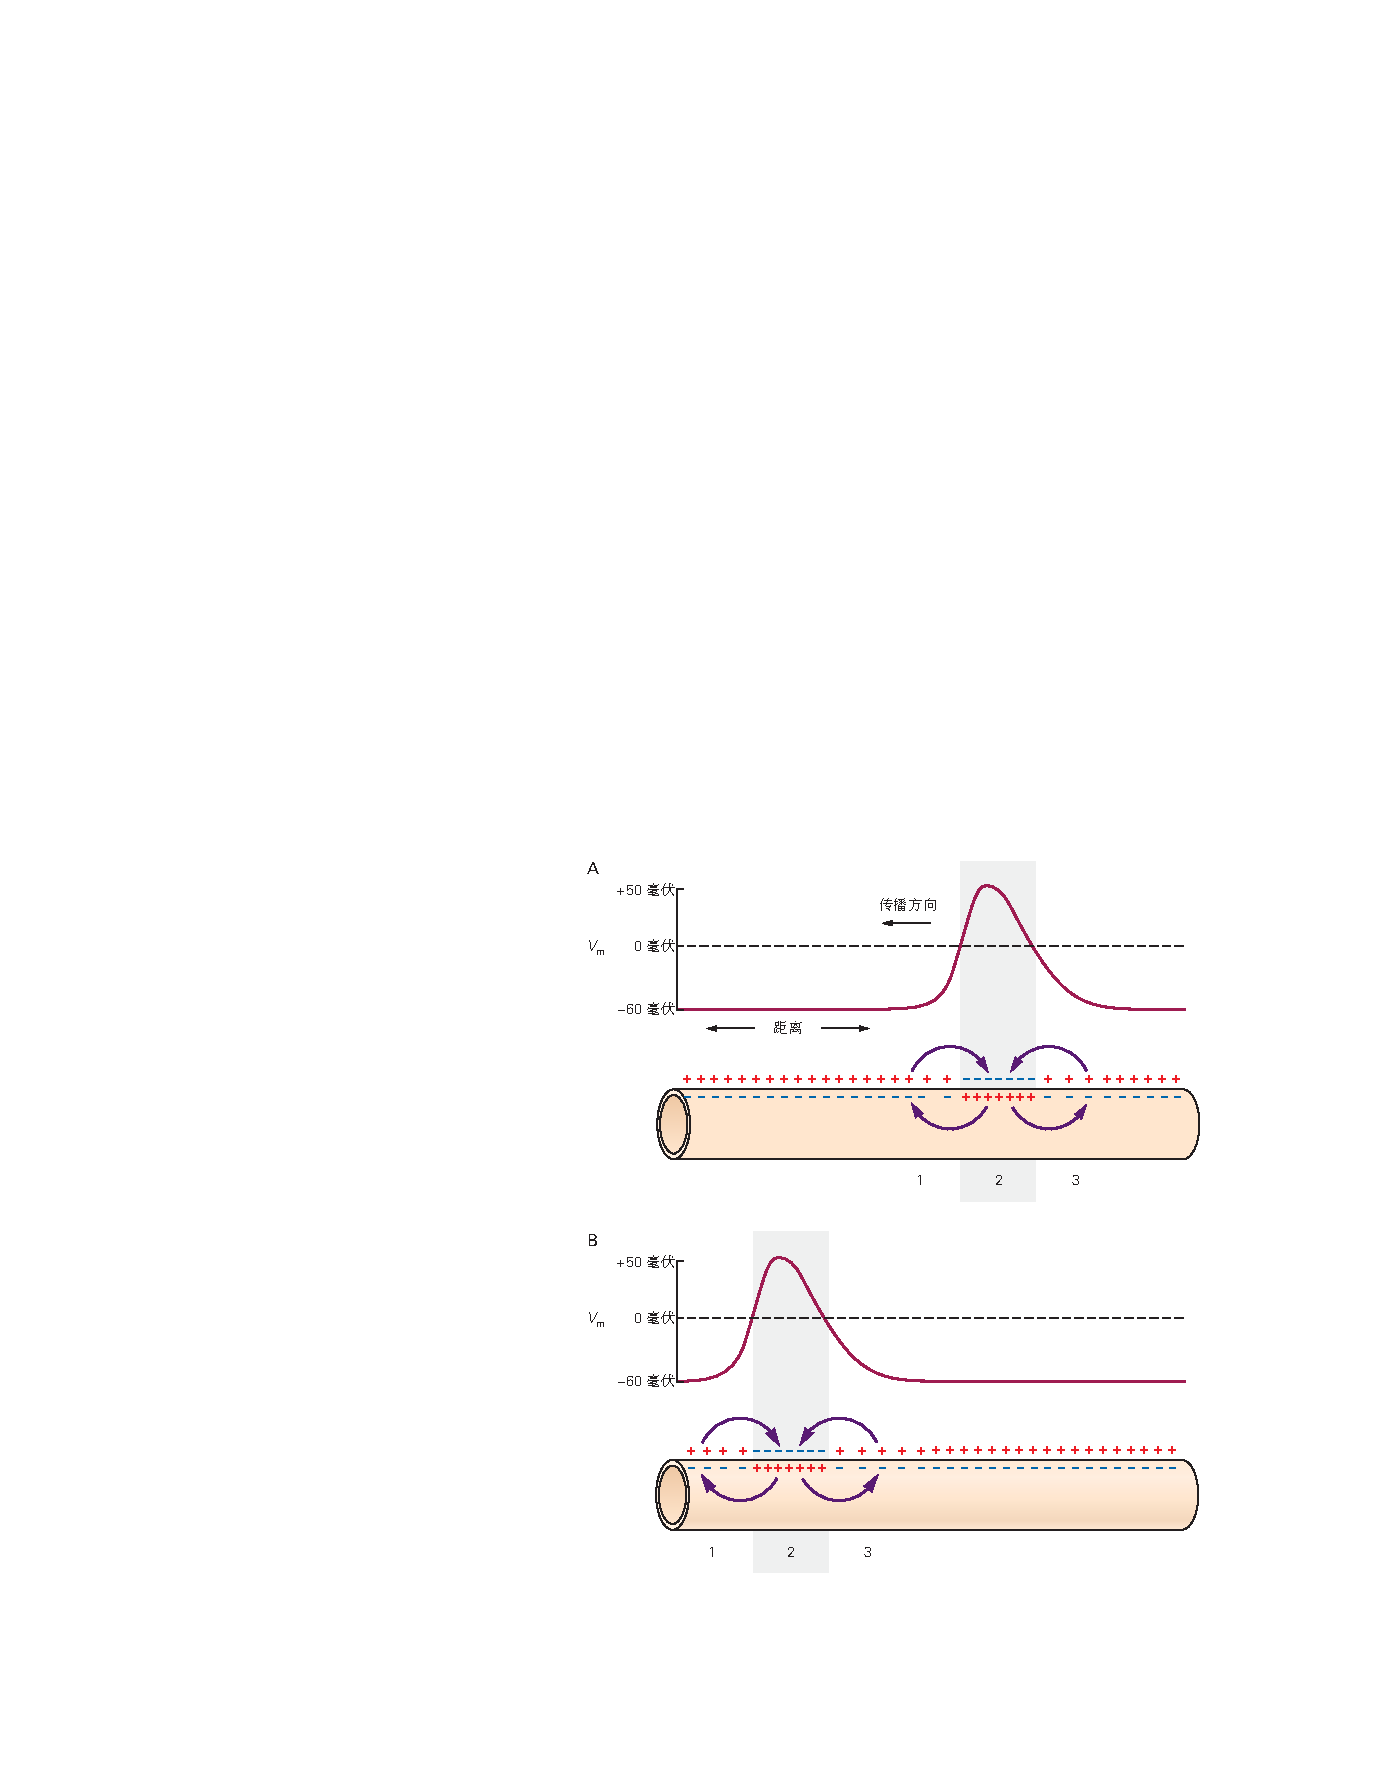
\includegraphics[width=0.7\linewidth]{chap09/fig_9_12}
	\caption{电紧张传导有助于动作电位的传播。 A. 从右向左传播的动作电位导致轴突两个相邻区域之间的膜电位差异。 这种差异会产生局部回路电流,导致去极化被动扩散。 电流从更积极的活动区域 (2) 传播到动作电位 (1) 之前的不太积极的静息区域,以及动作电位 (3) 后面的不太积极的区域。 然而,由于在动作电位之后膜 \ce{K+} 电导也增加(第 \ref{chap:chap10} 章),区域 3 中沿膜内侧的正电荷积累超过了局部 \ce{K+} 流出的平衡, 让这个膜区域重新极化。 B. 不久之后,动作电位沿轴突向下移动并重复该过程。}
	\label{fig:9_12}
\end{figure}



\subsection{大轴突比小轴突更容易兴奋}

轴突几何形状对动作电位传导的影响在常见的神经学检查中起着重要作用。
在对周围神经疾病患者进行检查时,通常通过放置在神经上的一对外部皮肤电极之间的电流来刺激神经,并记录由此产生的动作电位(复合动作电位)的数量。
神经通过第二对皮肤电压记录电极。
在这种情况下,产生动作电位的轴突总数随电流脉冲的幅度而变化(第~\ref{chap:chap57} 章)。


为了将细胞驱动到阈值,来自正电极的刺激电流必须穿过细胞膜进入轴突。
它在那里沿着轴浆核心行进,最终通过膜离开轴突进入细胞外液,到达第二个(负)电极。
然而,大部分刺激电流甚至不进入轴突,而是通过相邻的轴突或通过细胞外液的低电阻通路移动。
因此,电流最容易进入的轴突是最容易兴奋的轴突。


通常,直径最大的轴突具有最低的此类激发阈值。
轴突的直径越大,电流沿轴突流动的轴向阻力就越小,因为轴突每单位长度的电荷载体(离子)数量更多。
因为更多的电流进入较大的轴突,所以轴突比较小的轴突更有效地去极化。
由于这些原因,较大的轴突在低电流值下被招募;
直径较小的轴突仅在相对较大的电流强度下被募集。


较大的轴突传导得更快并且具有较低的激发电流阈值这一事实有助于解释临床神经刺激测试。
传递不同类型信息(例如,运动与感觉)的神经元通常轴突直径不同,因此传导速度也不同(第 ~\ref{chap:chap18}~章)。 
此外,特定疾病可能优先影响轴突的某些功能类别。
因此,使用传导速度作为确定哪类轴突具有缺陷传导特性的标准可以帮助人们推断神经功能缺损的神经元基础。



\subsection{被动膜特性和轴突直径影响动作电位传播速度}

动作电位传导期间去极化的被动扩散不是瞬时的。
事实上,电紧张传导是动作电位传播的限速因素。
我们可以通过考虑由一段轴浆连接的两个相邻轴突膜段的简化等效回路来理解这种限制。


在膜的一个片段中产生的动作电位向相邻的膜提供去极化电流,使其逐渐向阈值去极化(图~\ref{fig:9_12})。 
根据欧姆定律,轴浆电阻越大,相邻膜段之间的电流越小(I = V / R),因此改变相邻段膜电容上的电荷所需的时间越长。


回想一下,由于 ΔV = ΔQ/C,如果电流很小,膜电位变化缓慢,因为 ΔQ 等于电流的大小乘以时间,变化缓慢。
类似地,膜电容越大,必须在膜上沉积更多的电荷以改变跨膜的电势,因此电流需要更长的时间来产生给定的去极化。
因此,去极化沿轴突传播所需的时间由轴向电阻 ra 和轴突每单位长度的电容 cm(单位 F/cm)共同决定。 
电荷的被动扩散率与乘积 racm 成反比。
如果此产品减少,则被动扩散速率增加,动作电位传播更快。


动作电位的快速传播在功能上很重要,并且已经进化出两种适应来增加它。
一是轴突核心直径的增加。
由于 ra 与轴突直径的平方成正比,而 cm 与直径成正比,因此直径增加的净效应是 racm 的减少。
这种适应在乌贼的巨大轴突中发挥到了极致,其直径可达 1 毫米。
没有进化出更大的轴突,这大概是因为竞争需要保持神经元的尺寸较小,以便许多细胞可以装入有限的空间。


第二种提高传导速度的适应是髓鞘包裹轴突(第 ~\ref{chap:chap7}~章)。 
这个过程在功能上相当于将轴突膜的厚度增加 100 倍。 
因为平行板电容器(例如膜)的电容与绝缘层的厚度成反比,所以髓鞘形成会减少 cm,从而减少 racm。
每层髓磷脂都非常薄——只有 80 埃。
因此,髓鞘形成导致 racm 的减少比例远大于裸轴突核直径的相同增加,因为髓鞘中的多层膜导致 cm 的大幅减少,而整个轴突的增加相对较小直径。
出于这个原因,有髓轴突的传导比相同直径的无髓轴突更快。


在具有有髓轴突的神经元中,动作电位在轴突的无髓鞘起始段被触发。
通过该膜区域的内向电流可用于释放前方有髓轴突的电容。
尽管轴突的电容非常小(因为髓鞘绝缘),但从触发区沿轴突核心流下的电流量不足以使整个有髓轴突长度上的电容放电。


为了防止动作电位消失,髓鞘每隔 1 到 2 毫米就会被郎飞结中断,即长度约为 1 微米的裸露轴突膜片(第 ~\ref{chap:chap7}~章)。 
尽管每个节点处的膜面积非常小,但节点膜富含电压门控 \ce{Na+} 通道,因此可以响应轴突的去极化被动扩散而产生强烈的去极化内向 \ce{Na+} 电流。
因此,这些规则分布的节点会周期性地提高动作电位的幅度,防止其随距离衰减。


由于髓鞘的低电容,动作电位沿节间区域传播得非常快,当它穿过每个裸节点的高电容区域时会减慢。
因此,当动作电位沿轴突向下移动时,它会从一个节点快速跳到另一个节点(图~\ref{fig:9_13}A)。 
出于这个原因,据说有髓轴突中的动作电位通过跳动传导(来自拉丁语 saltare,跳跃)移动。
因为离子仅在有髓纤维的节点处穿过膜,所以从代谢的角度来看,跳跃式传导也是有利的。
\ce{Na+}-\ce{K+} 泵必须消耗更少的能量来恢复 \ce{Na+} 和 \ce{K+} 浓度梯度,随着动作电位的传播,\ce{Na+} 和 \ce{K+} 浓度梯度趋于下降。


\begin{figure}[htbp]
	\centering
	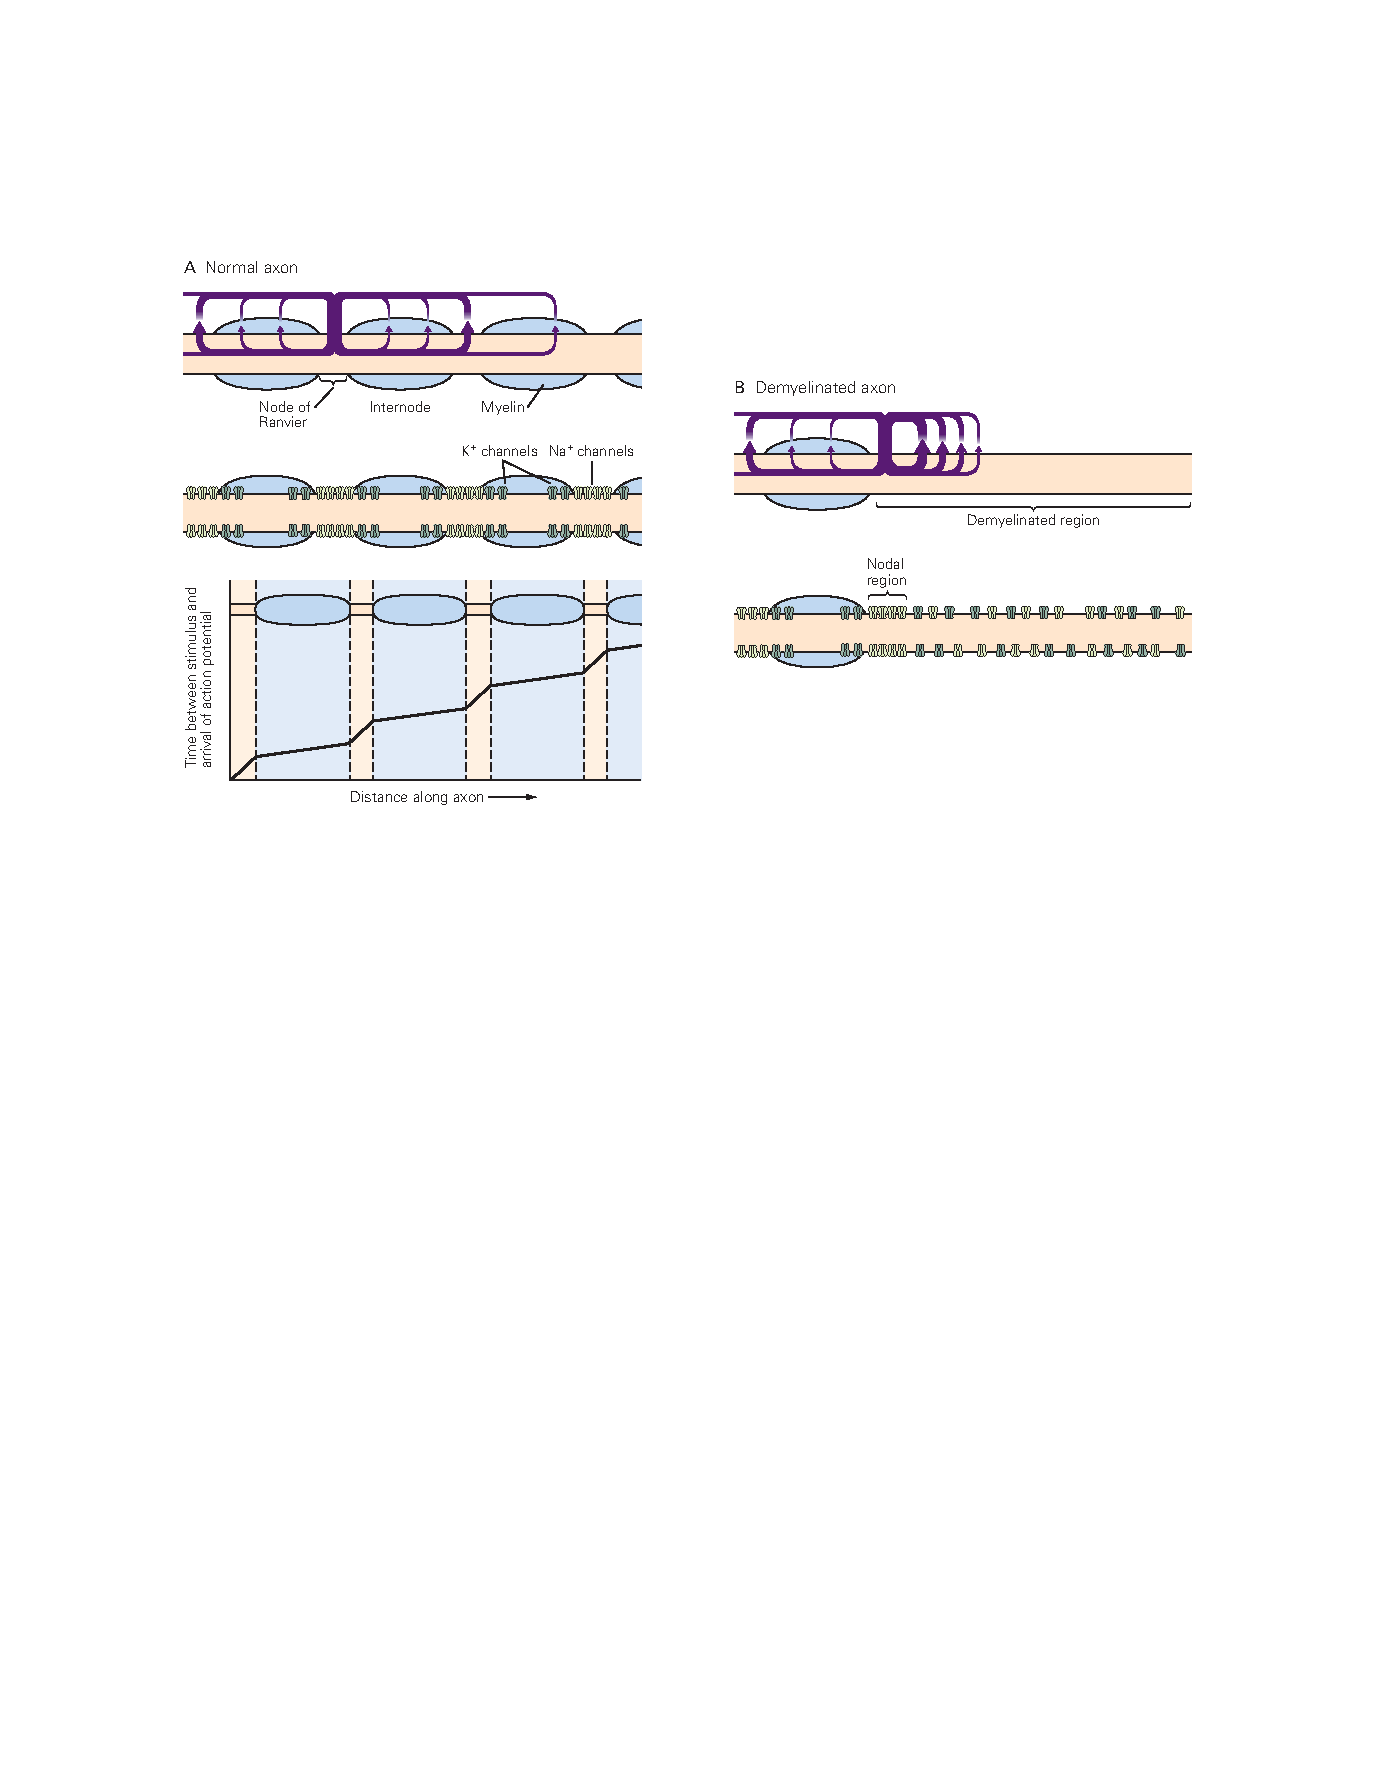
\includegraphics[width=0.5\linewidth]{chap09/fig_9_13}
	\caption{有髓神经中的动作电位在 Ranvier 节点处再生。 A. 电容和离子膜电流的密度(膜每单位面积的膜电流)在 Ranvier 节点处比髓鞘绝缘的节间区域高得多。 (沿轴突的任何点的膜电流密度由箭头的粗细表示。)由于轴突膜在节点处的电容较高,动作电位在接近每个节点时减慢,因此看起来跳跃 当它从左向右传播时,从一个节点快速传播到另一个节点。 B. 在失去髓鞘的轴突区域,动作电位的传播减慢或受阻。 局部回路电流必须释放更大的膜电容,并且由于长度常数较短(由轴突脱髓鞘延伸中的低膜电阻引起),它们不会沿轴突向下扩散。 为响应脱髓鞘,额外的电压门控 \ce{Na+} 和 \ce{K+} 离子通道被插入通常有髓鞘的膜中。}
	\label{fig:9_13}
\end{figure}


传导速度的分布在神经元之间甚至轴突的不同分支之间变化很大,这取决于轴突直径和髓鞘形成程度。
有髓轴突的其他几何特征,如节间长度和节直径,也会影响速度。
进化已经适应传导速度以优化每个神经元的行为功能。 
通常,参与快速感觉和运动计算的轴突通常具有高传导率。
更具体地说,在听觉系统的某些神经回路中,最佳行为反应取决于汇聚到同一突触后神经元的两条通路中突触前动作电位的精确时间关系(第~\ref{chap:chap28}~ 章)。
在这种情况下,两个输入路径中有髓轴突的几何参数值会导致不同的传导速度,以补偿输入路径长度的差异。


神经系统的各种疾病都是由脱髓鞘引起的,例如多发性硬化症和吉兰-巴利综合征。
当动作电位从有髓区域移动到裸露的脱髓鞘轴突时,它会遇到一个相对高 cm 和低 rm 的区域。
在脱髓鞘节段之前的节点处产生的内向电流可能太小,无法提供将脱髓鞘膜节段去极化至阈值所需的电容电流。
此外,该局部回路电流不会像正常情况下那样扩散,因为它遇到了一段轴突,由于其 rm 较低,该轴突的长度常数相对较短(图 \ref{fig:9_13}B)。
这两个因素可以结合起来减慢,在某些情况下实际上会阻止动作电位的传导,从而对行为造成破坏性影响(第 ~\ref{chap:chap57}~章)。

\section{亮点}

1. 当细胞处于静止状态时,离子通过离子通道进出细胞的被动通量是平衡的,因此跨膜的电荷分离保持恒定,膜电位保持在其静止值。 


2. 细胞膜对离子种类的渗透性与允许该离子通过的开放通道的数量成正比。
根据 Goldman 方程,神经细胞的静息膜电位值由传导 \ce{K+}、\ce{Cl-} 和 \ce{Na+} 的静息通道决定;
膜电位最接近具有最大膜渗透性的离子或离子的平衡(能斯特)电位。 


3. 产生神经元电信号(动作电位、突触电位和受体电位)的膜电位变化是由膜对这三种离子和钙离子离子的相对渗透性变化引起的。 


4. 虽然由门控离子通道打开引起的渗透性变化改变了跨膜的净电荷分离,但它们通常只对离子的体积浓度产生可忽略不计的变化。


5. 神经元的功能特性可以用等效回路来描述,包括膜电容、离子电导、离子通道的 EMF 产生特性和细胞质电阻。
在这个模型中,膜电位由具有最大膜电导的一个或多个离子决定。 


6. 离子泵防止离子电池由于通过离子通道的被动通量而耗尽。
\ce{Na+}-\ce{K+} 泵利用一个 ATP 分子的化学能将三个细胞内 \ce{Na+} 离子交换为两个细胞外 \ce{K+} 离子,这是初级主动运输的一个例子。
协同转运蛋白的二次主动转运是通过耦合一种或两种类型离子的下坡离子梯度来驱动另一种离子的上坡传输来提供动力的。
偶联可以采用同步传输(同向)或反传输(相反方向)的形式。 


7. \ce{Na+}-钙离子抗转运蛋白将内部钙离子离子交换为外部 \ce{Na+} 离子。
细胞膜中有两种类型的 \ce{Cl-} 协同转运蛋白。
将 Cl− 和 \ce{K+} 转运出细胞的 Cl−-\ce{K+} 共转运蛋白将 ECl 维持在相对负电位,是成熟神经元中发现的最常见的 Cl− 转运蛋白变体。
将 Cl–、\ce{Na+} 和 \ce{K+} 转运到细胞中的 Cl−-\ce{Na+}-\ce{K+} 共转运体产生相对正的 ECl。
它在未成熟神经元和某些成年神经元中表达。 


8. 初级和次级主动运输过程中分子转换的细节是一个积极研究的领域。


9. 神经细胞膜每单位膜面积具有相对较高的电容。
结果,当通道打开并且离子开始流动时,膜电位的变化比膜电流的变化更慢。


10. 改变沿轴突或树突长度的膜电容电荷的电流通过相对较差的导体——细胞质的细柱。
这两个因素结合在一起会减慢电压信号的传导速度。
此外,在静止时打开并产生静息电位的各种离子通道也会降低神经元的信号功能,因为它们会使细胞渗漏并限制信号被动传播的距离。 


11. 为了克服长距离信号的物理限制,神经元使用电压门控 \ce{Na+} 和 \ce{K+} 通道的顺序瞬态打开来产生动作电位。
动作电位沿着轴突不断再生,因此没有衰减地传导。 


12. 对于快速信号传导特别重要的通路,动作电位的传导通过轴突髓鞘化、轴突直径增加或两者兼有而增强。
传导速度可以在轴突之间或轴突内以优化神经元回路内神经元信号时间的方式变化。









